\documentclass[aspectratio=169]{beamer}
\usepackage[utf8]{inputenc}
\usepackage[T1]{fontenc}
\usepackage{amsmath,amssymb}
\usepackage{graphicx}
\usepackage{xcolor}
\usepackage{tikz}
\usetikzlibrary{arrows.meta,decorations.pathmorphing,calc}

%% Para ver las notas durante la presentación, usar pympress o pdfpc.
%% O descomentar para imprimir en segunda pantalla:
%% \setbeameroption{show notes on second screen=right}

% ---- TEMA ----
\usetheme{default}
\usecolortheme{default}

\definecolor{azul}{RGB}{10,50,100}
\definecolor{azulclaro}{RGB}{210,225,245}
\definecolor{rojo}{RGB}{150,25,25}
\definecolor{verde}{RGB}{20,100,55}
\definecolor{gris}{RGB}{90,90,90}

\setbeamercolor{structure}{fg=azul}
\setbeamercolor{frametitle}{bg=azul,fg=white}
\setbeamercolor{block title}{bg=azul,fg=white}
\setbeamercolor{block body}{bg=azulclaro}
\setbeamercolor{alerted text}{fg=rojo}
\setbeamerfont{frametitle}{series=\bfseries,size=\large}
\setbeamerfont{block title}{series=\bfseries}
\setbeamertemplate{navigation symbols}{}
\setbeamertemplate{footline}{%
	\hfill{\color{gris}\scriptsize\insertframenumber/19 \hspace{6pt}}%
	\vspace{4pt}%
}

% ---- COMANDOS ----
\newcommand{\vb}[1]{\mathbf{#1}}
\newcommand{\di}{\nabla\!\cdot}
\newcommand{\ro}{\nabla\!\times}
\newcommand{\rh}{\hat{\mathbf{r}}}
\newcommand{\rph}{\hat{\mathbf{r}}'}
\newcommand{\ph}{\hat{\boldsymbol{\varphi}}'}

% ---- PORTADA ----
\title[Monopolos de Dirac]{Observación de monopolos de Dirac\\en un campo magnético sintético}
\subtitle{M. W. Ray, E. Ruokokoski, S. Kandel, M. Möttönen \& D. S. Hall.}
\author{Simón Fonseca}
\date{Junio 2026}

\begin{document}
	
	% ==============================================================
	% 1. PORTADA
	% ==============================================================
	\begin{frame}
		\titlepage
	\end{frame}
	\note{
		Presentar brevemente. «Voy a hablar de un paper de Nature de 2014 que logró crear y observar, por primera vez, un monopolo de Dirac en un sistema cuántico controlado».
		Mencionar que es un resultado de electrodinámica clásica realizado en la práctica usando física de la materia condensada.
	}
	
	% ==============================================================
	% 2. MOTIVACIÓN — IMÁN CLÁSICO
	% ==============================================================
	\begin{frame}{Bipolaridad del campo magnético}
		\centering
		\vspace{-4pt}
		
		
		
		\tikzset{every picture/.style={line width=0.75pt}} %set default line width to 0.75pt        
		
		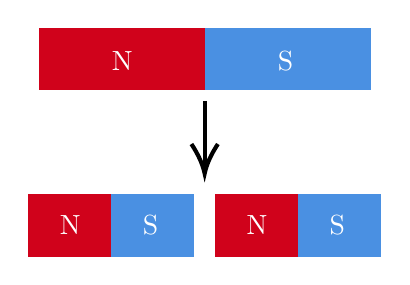
\begin{tikzpicture}[x=0.75pt,y=0.75pt,yscale=-1,xscale=1]
			%uncomment if require: \path (0,300); %set diagram left start at 0, and has height of 300
			
			%Shape: Rectangle [id:dp8488285764461364] 
			\draw  [draw opacity=0][fill={rgb, 255:red, 208; green, 2; blue, 27 }  ,fill opacity=1 ] (40,20) -- (120,20) -- (120,50) -- (40,50) -- cycle ;
			%Shape: Rectangle [id:dp11564086250695826] 
			\draw  [draw opacity=0][fill={rgb, 255:red, 74; green, 144; blue, 226 }  ,fill opacity=1 ] (120,20) -- (200,20) -- (200,50) -- (120,50) -- cycle ;
			%Shape: Rectangle [id:dp9081057124848559] 
			\draw  [draw opacity=0][fill={rgb, 255:red, 208; green, 2; blue, 27 }  ,fill opacity=1 ] (35,100) -- (75,100) -- (75,130) -- (35,130) -- cycle ;
			%Shape: Rectangle [id:dp43801470108948626] 
			\draw  [draw opacity=0][fill={rgb, 255:red, 74; green, 144; blue, 226 }  ,fill opacity=1 ] (75,100) -- (115,100) -- (115,130) -- (75,130) -- cycle ;
			%Shape: Rectangle [id:dp2701857688281072] 
			\draw  [draw opacity=0][fill={rgb, 255:red, 208; green, 2; blue, 27 }  ,fill opacity=1 ] (125,100) -- (165,100) -- (165,130) -- (125,130) -- cycle ;
			%Shape: Rectangle [id:dp5477819716167177] 
			\draw  [draw opacity=0][fill={rgb, 255:red, 74; green, 144; blue, 226 }  ,fill opacity=1 ] (165,100) -- (205,100) -- (205,130) -- (165,130) -- cycle ;
			%Straight Lines [id:da22775367624435305] 
			\draw [line width=1.5]    (120,55) -- (120,87) ;
			\draw [shift={(120,90)}, rotate = 270] [color={rgb, 255:red, 0; green, 0; blue, 0 }  ][line width=1.5]    (14.21,-6.37) .. controls (9.04,-2.99) and (4.3,-0.87) .. (0,0) .. controls (4.3,0.87) and (9.04,2.99) .. (14.21,6.37)   ;
			
			% Text Node
			\draw (74,30) node [anchor=north west][inner sep=0.75pt]  [color={rgb, 255:red, 255; green, 255; blue, 255 }  ,opacity=1 ] [align=left] {N};
			% Text Node
			\draw (49,109) node [anchor=north west][inner sep=0.75pt]  [color={rgb, 255:red, 255; green, 255; blue, 255 }  ,opacity=1 ] [align=left] {N};
			% Text Node
			\draw (139,109) node [anchor=north west][inner sep=0.75pt]  [color={rgb, 255:red, 255; green, 255; blue, 255 }  ,opacity=1 ] [align=left] {N};
			% Text Node
			\draw (154,30) node [anchor=north west][inner sep=0.75pt]  [color={rgb, 255:red, 255; green, 255; blue, 255 }  ,opacity=1 ] [align=left] {S};
			% Text Node
			\draw (89,109) node [anchor=north west][inner sep=0.75pt]  [color={rgb, 255:red, 255; green, 255; blue, 255 }  ,opacity=1 ] [align=left] {S};
			% Text Node
			\draw (179,109) node [anchor=north west][inner sep=0.75pt]  [color={rgb, 255:red, 255; green, 255; blue, 255 }  ,opacity=1 ] [align=left] {S};
			
			
		\end{tikzpicture}
		
		
		\vspace{8pt}
		\Large
		\[
		\di\vb{B} = 0
		\]
	\end{frame}
	\note{
		Recordar que en electromagnetismo ∇·B = 0 es una de las leyes de Maxwell.
		Esto significa que no existen cargas magnéticas: las líneas de campo siempre son cerradas.
		Si cortamos un imán, no obtenemos un polo Norte solo y un polo Sur solo: siempre vienen en pares.
		Preguntar retóricamente: ¿pero qué pasaría si pudiera existir un polo solo?
	}
	
	% ==============================================================
	% 3. ¿QUÉ SERÍA UN MONOPOLO?
	% ==============================================================
	\begin{frame}{Monopolo magnético}
		
		\begin{columns}[c]
			\begin{column}{0.45\textwidth}
				\centering
				
				
				\tikzset{every picture/.style={line width=0.75pt}} %set default line width to 0.75pt        
				
				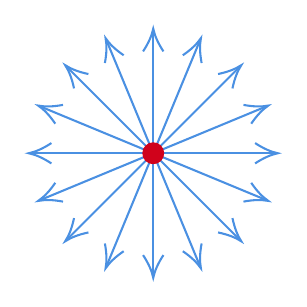
\begin{tikzpicture}[x=0.75pt,y=0.75pt,yscale=-1,xscale=1]
					%uncomment if require: \path (0,300); %set diagram left start at 0, and has height of 300
					
					%Straight Lines [id:da23143997447444586] 
					\draw [color={rgb, 255:red, 74; green, 144; blue, 226 }  ,draw opacity=1 ][line width=0.75]    (92.2,123.59) -- (47.8,16.41) ;
					\draw [shift={(47.04,14.57)}, rotate = 67.5] [color={rgb, 255:red, 74; green, 144; blue, 226 }  ,draw opacity=1 ][line width=0.75]    (10.93,-4.9) .. controls (6.95,-2.3) and (3.31,-0.67) .. (0,0) .. controls (3.31,0.67) and (6.95,2.3) .. (10.93,4.9)   ;
					\draw [shift={(92.96,125.43)}, rotate = 247.5] [color={rgb, 255:red, 74; green, 144; blue, 226 }  ,draw opacity=1 ][line width=0.75]    (10.93,-4.9) .. controls (6.95,-2.3) and (3.31,-0.67) .. (0,0) .. controls (3.31,0.67) and (6.95,2.3) .. (10.93,4.9)   ;
					%Straight Lines [id:da5220328590285531] 
					\draw [color={rgb, 255:red, 74; green, 144; blue, 226 }  ,draw opacity=1 ][line width=0.75]    (47.8,123.59) -- (92.2,16.41) ;
					\draw [shift={(92.96,14.57)}, rotate = 112.5] [color={rgb, 255:red, 74; green, 144; blue, 226 }  ,draw opacity=1 ][line width=0.75]    (10.93,-4.9) .. controls (6.95,-2.3) and (3.31,-0.67) .. (0,0) .. controls (3.31,0.67) and (6.95,2.3) .. (10.93,4.9)   ;
					\draw [shift={(47.04,125.43)}, rotate = 292.5] [color={rgb, 255:red, 74; green, 144; blue, 226 }  ,draw opacity=1 ][line width=0.75]    (10.93,-4.9) .. controls (6.95,-2.3) and (3.31,-0.67) .. (0,0) .. controls (3.31,0.67) and (6.95,2.3) .. (10.93,4.9)   ;
					%Straight Lines [id:da21409789243592459] 
					\draw [color={rgb, 255:red, 74; green, 144; blue, 226 }  ,draw opacity=1 ][line width=0.75]    (16.41,92.2) -- (123.59,47.8) ;
					\draw [shift={(125.43,47.04)}, rotate = 157.5] [color={rgb, 255:red, 74; green, 144; blue, 226 }  ,draw opacity=1 ][line width=0.75]    (10.93,-4.9) .. controls (6.95,-2.3) and (3.31,-0.67) .. (0,0) .. controls (3.31,0.67) and (6.95,2.3) .. (10.93,4.9)   ;
					\draw [shift={(14.57,92.96)}, rotate = 337.5] [color={rgb, 255:red, 74; green, 144; blue, 226 }  ,draw opacity=1 ][line width=0.75]    (10.93,-4.9) .. controls (6.95,-2.3) and (3.31,-0.67) .. (0,0) .. controls (3.31,0.67) and (6.95,2.3) .. (10.93,4.9)   ;
					%Straight Lines [id:da5645002661675905] 
					\draw [color={rgb, 255:red, 74; green, 144; blue, 226 }  ,draw opacity=1 ][line width=0.75]    (16.41,47.8) -- (123.59,92.2) ;
					\draw [shift={(125.43,92.96)}, rotate = 202.5] [color={rgb, 255:red, 74; green, 144; blue, 226 }  ,draw opacity=1 ][line width=0.75]    (10.93,-4.9) .. controls (6.95,-2.3) and (3.31,-0.67) .. (0,0) .. controls (3.31,0.67) and (6.95,2.3) .. (10.93,4.9)   ;
					\draw [shift={(14.57,47.04)}, rotate = 22.5] [color={rgb, 255:red, 74; green, 144; blue, 226 }  ,draw opacity=1 ][line width=0.75]    (10.93,-4.9) .. controls (6.95,-2.3) and (3.31,-0.67) .. (0,0) .. controls (3.31,0.67) and (6.95,2.3) .. (10.93,4.9)   ;
					%Straight Lines [id:da3401200219861904] 
					\draw [color={rgb, 255:red, 74; green, 144; blue, 226 }  ,draw opacity=1 ][line width=0.75]    (70,12) -- (70,128) ;
					\draw [shift={(70,130)}, rotate = 270] [color={rgb, 255:red, 74; green, 144; blue, 226 }  ,draw opacity=1 ][line width=0.75]    (10.93,-4.9) .. controls (6.95,-2.3) and (3.31,-0.67) .. (0,0) .. controls (3.31,0.67) and (6.95,2.3) .. (10.93,4.9)   ;
					\draw [shift={(70,10)}, rotate = 90] [color={rgb, 255:red, 74; green, 144; blue, 226 }  ,draw opacity=1 ][line width=0.75]    (10.93,-4.9) .. controls (6.95,-2.3) and (3.31,-0.67) .. (0,0) .. controls (3.31,0.67) and (6.95,2.3) .. (10.93,4.9)   ;
					%Straight Lines [id:da7901551066412535] 
					\draw [color={rgb, 255:red, 74; green, 144; blue, 226 }  ,draw opacity=1 ][line width=0.75]    (111.01,111.01) -- (28.99,28.99) ;
					\draw [shift={(27.57,27.57)}, rotate = 45] [color={rgb, 255:red, 74; green, 144; blue, 226 }  ,draw opacity=1 ][line width=0.75]    (10.93,-4.9) .. controls (6.95,-2.3) and (3.31,-0.67) .. (0,0) .. controls (3.31,0.67) and (6.95,2.3) .. (10.93,4.9)   ;
					\draw [shift={(112.43,112.43)}, rotate = 225] [color={rgb, 255:red, 74; green, 144; blue, 226 }  ,draw opacity=1 ][line width=0.75]    (10.93,-4.9) .. controls (6.95,-2.3) and (3.31,-0.67) .. (0,0) .. controls (3.31,0.67) and (6.95,2.3) .. (10.93,4.9)   ;
					%Straight Lines [id:da7583322038525004] 
					\draw [color={rgb, 255:red, 74; green, 144; blue, 226 }  ,draw opacity=1 ][line width=0.75]    (128,70) -- (12,70) ;
					\draw [shift={(10,70)}, rotate = 360] [color={rgb, 255:red, 74; green, 144; blue, 226 }  ,draw opacity=1 ][line width=0.75]    (10.93,-4.9) .. controls (6.95,-2.3) and (3.31,-0.67) .. (0,0) .. controls (3.31,0.67) and (6.95,2.3) .. (10.93,4.9)   ;
					\draw [shift={(130,70)}, rotate = 180] [color={rgb, 255:red, 74; green, 144; blue, 226 }  ,draw opacity=1 ][line width=0.75]    (10.93,-4.9) .. controls (6.95,-2.3) and (3.31,-0.67) .. (0,0) .. controls (3.31,0.67) and (6.95,2.3) .. (10.93,4.9)   ;
					%Straight Lines [id:da8096894207244196] 
					\draw [color={rgb, 255:red, 74; green, 144; blue, 226 }  ,draw opacity=1 ][line width=0.75]    (28.99,111.01) -- (111.01,28.99) ;
					\draw [shift={(112.43,27.57)}, rotate = 135] [color={rgb, 255:red, 74; green, 144; blue, 226 }  ,draw opacity=1 ][line width=0.75]    (10.93,-4.9) .. controls (6.95,-2.3) and (3.31,-0.67) .. (0,0) .. controls (3.31,0.67) and (6.95,2.3) .. (10.93,4.9)   ;
					\draw [shift={(27.57,112.43)}, rotate = 315] [color={rgb, 255:red, 74; green, 144; blue, 226 }  ,draw opacity=1 ][line width=0.75]    (10.93,-4.9) .. controls (6.95,-2.3) and (3.31,-0.67) .. (0,0) .. controls (3.31,0.67) and (6.95,2.3) .. (10.93,4.9)   ;
					%Shape: Circle [id:dp03695235929793517] 
					\draw  [color={rgb, 255:red, 208; green, 2; blue, 27 }  ,draw opacity=1 ][fill={rgb, 255:red, 208; green, 2; blue, 27 }  ,fill opacity=1 ] (65,70) .. controls (65,67.24) and (67.24,65) .. (70,65) .. controls (72.76,65) and (75,67.24) .. (75,70) .. controls (75,72.76) and (72.76,75) .. (70,75) .. controls (67.24,75) and (65,72.76) .. (65,70) -- cycle ;
					
					
					
					
				\end{tikzpicture}
				
			\end{column}
			\begin{column}{0.52\textwidth}
				\[
				\di\vb{B} = \rho_M
				\quad\Rightarrow\quad
				\vb{B} = \frac{g}{r^2}\rh
				\]
				\vspace{10pt}
				\begin{block}{Consecuencia}
					\centering
					Si existe \emph{al menos uno}:
					\[
					\boxed{qg = \frac{n\hbar c}{2}}
					\]
					Toda carga eléctrica está cuantizada.
				\end{block}
			\end{column}
		\end{columns}
	\end{frame}
	\note{
		Un monopolo magnético sería una partícula que se comporta como un polo Norte (o Sur) aislado.
		El campo que generaría sería como el campo de Coulomb pero para magnetismo: B = g r̂/r².
		Dirac mostró en 1931 que si existiera al menos un monopolo de carga g en el universo, la condición qg = nℏc/2 implicaría que todas las cargas eléctricas deben ser múltiplos enteros de ℏc/2g.
		Esto explicaría por qué todas las cargas observadas son múltiplos de la carga del electrón — algo que hoy damos por sentado pero que la electrodinámica clásica no explica.
	}
	
	% ==============================================================
	% 4. EL PROBLEMA MATEMÁTICO
	% ==============================================================
	\begin{frame}{Potencial vectorial}
		
		\centering
		\vspace{8pt}
		
		\Large
		\begin{equation*}
			\vb{B} = \ro\vb{A}
			\quad\Longrightarrow\quad
			\di\vb{B} = \di(\ro\vb{A}) \equiv 0
		\end{equation*}
		
		\vspace{20pt}
		\normalsize
		\begin{alertblock}{\centering Identidad vectorial}
			\centering
			El potencial vectorial $\vb{A}$ globalmente bien definido
			es \emph{incompatible} con un monopolo.\\[4pt]
			La mecánica cuántica exige $\vb{A}$ (efecto Aharonov-Bohm).
		\end{alertblock}
		
	\end{frame}
	\note{
		Esta es la razón por la que el monopolo es un problema en física teórica.
		En mecánica cuántica el Hamiltoniano se escribe en términos de A, no de B directamente.
		El efecto Aharonov-Bohm (que vimos en el curso) demuestra que A tiene efectos físicos reales incluso donde B=0.
		Entonces si queremos un monopolo, necesitamos A, pero A siempre nos da ∇·B = 0. Parece un callejón sin salida.
		Dirac encontró la salida permitiendo que A sea singular en una línea.
	}
	
	% ==============================================================
	% 5. LA SOLUCIÓN DE DIRAC — DIRAC STRING
	% ==============================================================
	\begin{frame}{\textit{Dirac string}}
		
		\begin{columns}[c]
			\begin{column}{0.44\textwidth}
				\centering
				
				
				\tikzset{every picture/.style={line width=0.75pt}} %set default line width to 0.75pt        
				
				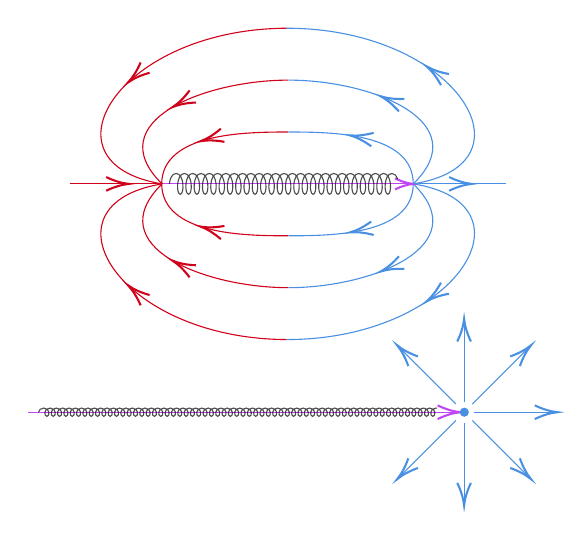
\begin{tikzpicture}[x=0.75pt,y=0.75pt,yscale=-1,xscale=1]
					%uncomment if require: \path (0,253); %set diagram left start at 0, and has height of 253
					
					%Straight Lines [id:da18687793493999383] 
					\draw [color={rgb, 255:red, 193; green, 70; blue, 241 }  ,draw opacity=1 ]   (35,205) -- (241.17,205) ;
					\draw [shift={(243.17,205)}, rotate = 180] [color={rgb, 255:red, 193; green, 70; blue, 241 }  ,draw opacity=1 ][line width=0.75]    (10.93,-3.29) .. controls (6.95,-1.4) and (3.31,-0.3) .. (0,0) .. controls (3.31,0.3) and (6.95,1.4) .. (10.93,3.29)   ;
					%Shape: Spring [id:dp9313734346311904] 
					\draw  [color={rgb, 255:red, 0; green, 0; blue, 0 }  ,draw opacity=0.7 ] (40,205) .. controls (40.19,204) and (40.95,203) .. (42.48,203) .. controls (45.52,203) and (45.52,207) .. (44,207) .. controls (42.48,207) and (42.48,203) .. (45.52,203) .. controls (48.57,203) and (48.57,207) .. (47.05,207) .. controls (45.52,207) and (45.52,203) .. (48.57,203) .. controls (51.62,203) and (51.62,207) .. (50.1,207) .. controls (48.57,207) and (48.57,203) .. (51.62,203) .. controls (54.67,203) and (54.67,207) .. (53.15,207) .. controls (51.62,207) and (51.62,203) .. (54.67,203) .. controls (57.72,203) and (57.72,207) .. (56.19,207) .. controls (54.67,207) and (54.67,203) .. (57.72,203) .. controls (60.77,203) and (60.77,207) .. (59.24,207) .. controls (57.72,207) and (57.72,203) .. (60.77,203) .. controls (63.81,203) and (63.81,207) .. (62.29,207) .. controls (60.77,207) and (60.77,203) .. (63.81,203) .. controls (66.86,203) and (66.86,207) .. (65.34,207) .. controls (63.81,207) and (63.81,203) .. (66.86,203) .. controls (69.91,203) and (69.91,207) .. (68.39,207) .. controls (66.86,207) and (66.86,203) .. (69.91,203) .. controls (72.96,203) and (72.96,207) .. (71.43,207) .. controls (69.91,207) and (69.91,203) .. (72.96,203) .. controls (76.01,203) and (76.01,207) .. (74.48,207) .. controls (72.96,207) and (72.96,203) .. (76.01,203) .. controls (79.06,203) and (79.06,207) .. (77.53,207) .. controls (76.01,207) and (76.01,203) .. (79.06,203) .. controls (82.1,203) and (82.1,207) .. (80.58,207) .. controls (79.06,207) and (79.06,203) .. (82.1,203) .. controls (85.15,203) and (85.15,207) .. (83.63,207) .. controls (82.1,207) and (82.1,203) .. (85.15,203) .. controls (88.2,203) and (88.2,207) .. (86.68,207) .. controls (85.15,207) and (85.15,203) .. (88.2,203) .. controls (91.25,203) and (91.25,207) .. (89.72,207) .. controls (88.2,207) and (88.2,203) .. (91.25,203) .. controls (94.3,203) and (94.3,207) .. (92.77,207) .. controls (91.25,207) and (91.25,203) .. (94.3,203) .. controls (97.34,203) and (97.34,207) .. (95.82,207) .. controls (94.3,207) and (94.3,203) .. (97.34,203) .. controls (100.39,203) and (100.39,207) .. (98.87,207) .. controls (97.34,207) and (97.34,203) .. (100.39,203) .. controls (103.44,203) and (103.44,207) .. (101.92,207) .. controls (100.39,207) and (100.39,203) .. (103.44,203) .. controls (106.49,203) and (106.49,207) .. (104.96,207) .. controls (103.44,207) and (103.44,203) .. (106.49,203) .. controls (109.54,203) and (109.54,207) .. (108.01,207) .. controls (106.49,207) and (106.49,203) .. (109.54,203) .. controls (112.59,203) and (112.59,207) .. (111.06,207) .. controls (109.54,207) and (109.54,203) .. (112.59,203) .. controls (115.63,203) and (115.63,207) .. (114.11,207) .. controls (112.59,207) and (112.59,203) .. (115.63,203) .. controls (118.68,203) and (118.68,207) .. (117.16,207) .. controls (115.63,207) and (115.63,203) .. (118.68,203) .. controls (121.73,203) and (121.73,207) .. (120.21,207) .. controls (118.68,207) and (118.68,203) .. (121.73,203) .. controls (124.78,203) and (124.78,207) .. (123.25,207) .. controls (121.73,207) and (121.73,203) .. (124.78,203) .. controls (127.83,203) and (127.83,207) .. (126.3,207) .. controls (124.78,207) and (124.78,203) .. (127.83,203) .. controls (130.87,203) and (130.87,207) .. (129.35,207) .. controls (127.83,207) and (127.83,203) .. (130.87,203) .. controls (133.92,203) and (133.92,207) .. (132.4,207) .. controls (130.87,207) and (130.87,203) .. (133.92,203) .. controls (136.97,203) and (136.97,207) .. (135.45,207) .. controls (133.92,207) and (133.92,203) .. (136.97,203) .. controls (140.02,203) and (140.02,207) .. (138.49,207) .. controls (136.97,207) and (136.97,203) .. (140.02,203) .. controls (143.07,203) and (143.07,207) .. (141.54,207) .. controls (140.02,207) and (140.02,203) .. (143.07,203) .. controls (146.12,203) and (146.12,207) .. (144.59,207) .. controls (143.07,207) and (143.07,203) .. (146.12,203) .. controls (149.16,203) and (149.16,207) .. (147.64,207) .. controls (146.12,207) and (146.12,203) .. (149.16,203) .. controls (152.21,203) and (152.21,207) .. (150.69,207) .. controls (149.16,207) and (149.16,203) .. (152.21,203) .. controls (155.26,203) and (155.26,207) .. (153.74,207) .. controls (152.21,207) and (152.21,203) .. (155.26,203) .. controls (158.31,203) and (158.31,207) .. (156.78,207) .. controls (155.26,207) and (155.26,203) .. (158.31,203) .. controls (161.36,203) and (161.36,207) .. (159.83,207) .. controls (158.31,207) and (158.31,203) .. (161.36,203) .. controls (164.4,203) and (164.4,207) .. (162.88,207) .. controls (161.36,207) and (161.36,203) .. (164.4,203) .. controls (167.45,203) and (167.45,207) .. (165.93,207) .. controls (164.4,207) and (164.4,203) .. (167.45,203) .. controls (170.5,203) and (170.5,207) .. (168.98,207) .. controls (167.45,207) and (167.45,203) .. (170.5,203) .. controls (173.55,203) and (173.55,207) .. (172.03,207) .. controls (170.5,207) and (170.5,203) .. (173.55,203) .. controls (176.6,203) and (176.6,207) .. (175.07,207) .. controls (173.55,207) and (173.55,203) .. (176.6,203) .. controls (179.65,203) and (179.65,207) .. (178.12,207) .. controls (176.6,207) and (176.6,203) .. (179.65,203) .. controls (182.69,203) and (182.69,207) .. (181.17,207) .. controls (179.65,207) and (179.65,203) .. (182.69,203) .. controls (185.74,203) and (185.74,207) .. (184.22,207) .. controls (182.69,207) and (182.69,203) .. (185.74,203) .. controls (188.79,203) and (188.79,207) .. (187.27,207) .. controls (185.74,207) and (185.74,203) .. (188.79,203) .. controls (191.84,203) and (191.84,207) .. (190.31,207) .. controls (188.79,207) and (188.79,203) .. (191.84,203) .. controls (194.89,203) and (194.89,207) .. (193.36,207) .. controls (191.84,207) and (191.84,203) .. (194.89,203) .. controls (197.93,203) and (197.93,207) .. (196.41,207) .. controls (194.89,207) and (194.89,203) .. (197.93,203) .. controls (200.98,203) and (200.98,207) .. (199.46,207) .. controls (197.93,207) and (197.93,203) .. (200.98,203) .. controls (204.03,203) and (204.03,207) .. (202.51,207) .. controls (200.98,207) and (200.98,203) .. (204.03,203) .. controls (207.08,203) and (207.08,207) .. (205.56,207) .. controls (204.03,207) and (204.03,203) .. (207.08,203) .. controls (210.13,203) and (210.13,207) .. (208.6,207) .. controls (207.08,207) and (207.08,203) .. (210.13,203) .. controls (213.18,203) and (213.18,207) .. (211.65,207) .. controls (210.13,207) and (210.13,203) .. (213.18,203) .. controls (216.22,203) and (216.22,207) .. (214.7,207) .. controls (213.18,207) and (213.18,203) .. (216.22,203) .. controls (219.27,203) and (219.27,207) .. (217.75,207) .. controls (216.22,207) and (216.22,203) .. (219.27,203) .. controls (222.32,203) and (222.32,207) .. (220.8,207) .. controls (219.27,207) and (219.27,203) .. (222.32,203) .. controls (225.37,203) and (225.37,207) .. (223.84,207) .. controls (222.32,207) and (222.32,203) .. (225.37,203) .. controls (228.42,203) and (228.42,207) .. (226.89,207) .. controls (225.37,207) and (225.37,203) .. (228.42,203) .. controls (231.47,203) and (231.47,207) .. (229.94,207) .. controls (228.42,207) and (228.42,203) .. (231.47,203) .. controls (231.66,203) and (231.83,203.02) .. (232,203.04) ;
					%Shape: Circle [id:dp9976515953764042] 
					\draw  [color={rgb, 255:red, 74; green, 144; blue, 226 }  ,draw opacity=1 ][fill={rgb, 255:red, 74; green, 144; blue, 226 }  ,fill opacity=1 ] (243.17,205) .. controls (243.17,203.94) and (244.02,203.08) .. (245.08,203.08) .. controls (246.14,203.08) and (247,203.94) .. (247,205) .. controls (247,206.06) and (246.14,206.92) .. (245.08,206.92) .. controls (244.02,206.92) and (243.17,206.06) .. (243.17,205) -- cycle ;
					%Straight Lines [id:da9803337688140109] 
					\draw [color={rgb, 255:red, 74; green, 144; blue, 226 }  ,draw opacity=1 ]   (245,200) -- (245,162) ;
					\draw [shift={(245,160)}, rotate = 90] [color={rgb, 255:red, 74; green, 144; blue, 226 }  ,draw opacity=1 ][line width=0.75]    (10.93,-3.29) .. controls (6.95,-1.4) and (3.31,-0.3) .. (0,0) .. controls (3.31,0.3) and (6.95,1.4) .. (10.93,3.29)   ;
					%Straight Lines [id:da02594517737390256] 
					\draw [color={rgb, 255:red, 74; green, 144; blue, 226 }  ,draw opacity=1 ]   (245,210) -- (245,248) ;
					\draw [shift={(245,250)}, rotate = 270] [color={rgb, 255:red, 74; green, 144; blue, 226 }  ,draw opacity=1 ][line width=0.75]    (10.93,-3.29) .. controls (6.95,-1.4) and (3.31,-0.3) .. (0,0) .. controls (3.31,0.3) and (6.95,1.4) .. (10.93,3.29)   ;
					%Straight Lines [id:da856741703681731] 
					\draw [color={rgb, 255:red, 74; green, 144; blue, 226 }  ,draw opacity=1 ]   (250,205) -- (288,205) ;
					\draw [shift={(290,205)}, rotate = 180] [color={rgb, 255:red, 74; green, 144; blue, 226 }  ,draw opacity=1 ][line width=0.75]    (10.93,-3.29) .. controls (6.95,-1.4) and (3.31,-0.3) .. (0,0) .. controls (3.31,0.3) and (6.95,1.4) .. (10.93,3.29)   ;
					%Straight Lines [id:da6378559154003527] 
					\draw [color={rgb, 255:red, 74; green, 144; blue, 226 }  ,draw opacity=1 ]   (249,209) -- (275.87,235.87) ;
					\draw [shift={(277.28,237.28)}, rotate = 225] [color={rgb, 255:red, 74; green, 144; blue, 226 }  ,draw opacity=1 ][line width=0.75]    (10.93,-3.29) .. controls (6.95,-1.4) and (3.31,-0.3) .. (0,0) .. controls (3.31,0.3) and (6.95,1.4) .. (10.93,3.29)   ;
					%Straight Lines [id:da5620212525131404] 
					\draw [color={rgb, 255:red, 74; green, 144; blue, 226 }  ,draw opacity=1 ]   (249,201) -- (275.87,174.13) ;
					\draw [shift={(277.28,172.72)}, rotate = 135] [color={rgb, 255:red, 74; green, 144; blue, 226 }  ,draw opacity=1 ][line width=0.75]    (10.93,-3.29) .. controls (6.95,-1.4) and (3.31,-0.3) .. (0,0) .. controls (3.31,0.3) and (6.95,1.4) .. (10.93,3.29)   ;
					%Straight Lines [id:da915339395493542] 
					\draw [color={rgb, 255:red, 74; green, 144; blue, 226 }  ,draw opacity=1 ]   (241,209) -- (214.13,235.87) ;
					\draw [shift={(212.72,237.28)}, rotate = 315] [color={rgb, 255:red, 74; green, 144; blue, 226 }  ,draw opacity=1 ][line width=0.75]    (10.93,-3.29) .. controls (6.95,-1.4) and (3.31,-0.3) .. (0,0) .. controls (3.31,0.3) and (6.95,1.4) .. (10.93,3.29)   ;
					%Straight Lines [id:da061391798493468874] 
					\draw [color={rgb, 255:red, 74; green, 144; blue, 226 }  ,draw opacity=1 ]   (241,201) -- (214.13,174.13) ;
					\draw [shift={(212.72,172.72)}, rotate = 45] [color={rgb, 255:red, 74; green, 144; blue, 226 }  ,draw opacity=1 ][line width=0.75]    (10.93,-3.29) .. controls (6.95,-1.4) and (3.31,-0.3) .. (0,0) .. controls (3.31,0.3) and (6.95,1.4) .. (10.93,3.29)   ;
					%Curve Lines [id:da16717545126305844] 
					\draw [color={rgb, 255:red, 74; green, 144; blue, 226 }  ,draw opacity=1 ]   (220.49,95) .. controls (220.49,70.33) and (181.09,70) .. (160.4,70) ;
					\draw [shift={(190.09,71.64)}, rotate = 10.45] [color={rgb, 255:red, 74; green, 144; blue, 226 }  ,draw opacity=1 ][line width=0.75]    (10.93,-3.29) .. controls (6.95,-1.4) and (3.31,-0.3) .. (0,0) .. controls (3.31,0.3) and (6.95,1.4) .. (10.93,3.29)   ;
					%Curve Lines [id:da37745831040244837] 
					\draw [color={rgb, 255:red, 208; green, 2; blue, 27 }  ,draw opacity=1 ]   (160.39,70) .. controls (139.68,70) and (99.62,70.33) .. (99.28,95) ;
					\draw [shift={(118.12,74.41)}, rotate = 344.92] [color={rgb, 255:red, 208; green, 2; blue, 27 }  ,draw opacity=1 ][line width=0.75]    (10.93,-3.29) .. controls (6.95,-1.4) and (3.31,-0.3) .. (0,0) .. controls (3.31,0.3) and (6.95,1.4) .. (10.93,3.29)   ;
					%Curve Lines [id:da3021684581706918] 
					\draw [color={rgb, 255:red, 74; green, 144; blue, 226 }  ,draw opacity=1 ]   (220.49,95) .. controls (251.02,65.33) and (201.11,45) .. (160.4,45) ;
					\draw [shift={(204.83,52.79)}, rotate = 23.09] [color={rgb, 255:red, 74; green, 144; blue, 226 }  ,draw opacity=1 ][line width=0.75]    (10.93,-3.29) .. controls (6.95,-1.4) and (3.31,-0.3) .. (0,0) .. controls (3.31,0.3) and (6.95,1.4) .. (10.93,3.29)   ;
					%Curve Lines [id:da2765798620623309] 
					\draw [color={rgb, 255:red, 208; green, 2; blue, 27 }  ,draw opacity=1 ]   (160.39,45) .. controls (119.99,45) and (68.92,65) .. (99.47,95) ;
					\draw [shift={(104.61,57.97)}, rotate = 332.27] [color={rgb, 255:red, 208; green, 2; blue, 27 }  ,draw opacity=1 ][line width=0.75]    (10.93,-3.29) .. controls (6.95,-1.4) and (3.31,-0.3) .. (0,0) .. controls (3.31,0.3) and (6.95,1.4) .. (10.93,3.29)   ;
					%Curve Lines [id:da9016106379080976] 
					\draw [color={rgb, 255:red, 208; green, 2; blue, 27 }  ,draw opacity=1 ]   (159.53,20) .. controls (78.38,20.33) and (38.7,85) .. (99.47,95) ;
					\draw [shift={(83.06,46.15)}, rotate = 319.01] [color={rgb, 255:red, 208; green, 2; blue, 27 }  ,draw opacity=1 ][line width=0.75]    (10.93,-3.29) .. controls (6.95,-1.4) and (3.31,-0.3) .. (0,0) .. controls (3.31,0.3) and (6.95,1.4) .. (10.93,3.29)   ;
					%Curve Lines [id:da27806999581454106] 
					\draw [color={rgb, 255:red, 74; green, 144; blue, 226 }  ,draw opacity=1 ]   (220.49,95) .. controls (281.56,85.33) and (241.3,20) .. (159.53,20) ;
					\draw [shift={(226.89,38.36)}, rotate = 35.68] [color={rgb, 255:red, 74; green, 144; blue, 226 }  ,draw opacity=1 ][line width=0.75]    (10.93,-3.29) .. controls (6.95,-1.4) and (3.31,-0.3) .. (0,0) .. controls (3.31,0.3) and (6.95,1.4) .. (10.93,3.29)   ;
					%Curve Lines [id:da3495970104110592] 
					\draw [color={rgb, 255:red, 74; green, 144; blue, 226 }  ,draw opacity=1 ]   (220.49,95) .. controls (220.49,119.67) and (181.09,120) .. (160.4,120) ;
					\draw [shift={(190.09,118.36)}, rotate = 349.55] [color={rgb, 255:red, 74; green, 144; blue, 226 }  ,draw opacity=1 ][line width=0.75]    (10.93,-3.29) .. controls (6.95,-1.4) and (3.31,-0.3) .. (0,0) .. controls (3.31,0.3) and (6.95,1.4) .. (10.93,3.29)   ;
					%Curve Lines [id:da7284548626546407] 
					\draw [color={rgb, 255:red, 208; green, 2; blue, 27 }  ,draw opacity=1 ]   (160.39,120) .. controls (139.68,120) and (99.62,119.67) .. (99.28,95) ;
					\draw [shift={(118.12,115.59)}, rotate = 15.08] [color={rgb, 255:red, 208; green, 2; blue, 27 }  ,draw opacity=1 ][line width=0.75]    (10.93,-3.29) .. controls (6.95,-1.4) and (3.31,-0.3) .. (0,0) .. controls (3.31,0.3) and (6.95,1.4) .. (10.93,3.29)   ;
					%Curve Lines [id:da5778581763345861] 
					\draw [color={rgb, 255:red, 74; green, 144; blue, 226 }  ,draw opacity=1 ]   (220.49,95) .. controls (251.02,124.67) and (201.11,145) .. (160.4,145) ;
					\draw [shift={(204.83,137.21)}, rotate = 336.91] [color={rgb, 255:red, 74; green, 144; blue, 226 }  ,draw opacity=1 ][line width=0.75]    (10.93,-3.29) .. controls (6.95,-1.4) and (3.31,-0.3) .. (0,0) .. controls (3.31,0.3) and (6.95,1.4) .. (10.93,3.29)   ;
					%Curve Lines [id:da11947915063843328] 
					\draw [color={rgb, 255:red, 208; green, 2; blue, 27 }  ,draw opacity=1 ]   (160.39,145) .. controls (119.99,145) and (68.92,125) .. (99.47,95) ;
					\draw [shift={(104.61,132.03)}, rotate = 27.73] [color={rgb, 255:red, 208; green, 2; blue, 27 }  ,draw opacity=1 ][line width=0.75]    (10.93,-3.29) .. controls (6.95,-1.4) and (3.31,-0.3) .. (0,0) .. controls (3.31,0.3) and (6.95,1.4) .. (10.93,3.29)   ;
					%Curve Lines [id:da3242148828513033] 
					\draw [color={rgb, 255:red, 208; green, 2; blue, 27 }  ,draw opacity=1 ]   (159.53,170) .. controls (78.38,169.67) and (38.7,105) .. (99.47,95) ;
					\draw [shift={(83.06,143.85)}, rotate = 40.99] [color={rgb, 255:red, 208; green, 2; blue, 27 }  ,draw opacity=1 ][line width=0.75]    (10.93,-3.29) .. controls (6.95,-1.4) and (3.31,-0.3) .. (0,0) .. controls (3.31,0.3) and (6.95,1.4) .. (10.93,3.29)   ;
					%Curve Lines [id:da9582388128377107] 
					\draw [color={rgb, 255:red, 74; green, 144; blue, 226 }  ,draw opacity=1 ]   (220.49,95) .. controls (281.56,104.67) and (241.3,170) .. (159.53,170) ;
					\draw [shift={(226.89,151.64)}, rotate = 324.32] [color={rgb, 255:red, 74; green, 144; blue, 226 }  ,draw opacity=1 ][line width=0.75]    (10.93,-3.29) .. controls (6.95,-1.4) and (3.31,-0.3) .. (0,0) .. controls (3.31,0.3) and (6.95,1.4) .. (10.93,3.29)   ;
					%Straight Lines [id:da4262140009507167] 
					\draw [color={rgb, 255:red, 193; green, 70; blue, 241 }  ,draw opacity=1 ]   (99.28,95) -- (218.49,95) ;
					\draw [shift={(220.49,95)}, rotate = 180] [color={rgb, 255:red, 193; green, 70; blue, 241 }  ,draw opacity=1 ][line width=0.75]    (8.74,-2.63) .. controls (5.56,-1.12) and (2.65,-0.24) .. (0,0) .. controls (2.65,0.24) and (5.56,1.12) .. (8.74,2.63)   ;
					%Shape: Spring [id:dp9846076555897383] 
					\draw  [color={rgb, 255:red, 0; green, 0; blue, 0 }  ,draw opacity=0.7 ] (103,95) .. controls (103.25,92.5) and (104.25,90) .. (106.25,90) .. controls (110.25,90) and (110.25,100) .. (108.25,100) .. controls (106.25,100) and (106.25,90) .. (110.25,90) .. controls (114.25,90) and (114.25,100) .. (112.25,100) .. controls (110.25,100) and (110.25,90) .. (114.25,90) .. controls (118.25,90) and (118.25,100) .. (116.25,100) .. controls (114.25,100) and (114.25,90) .. (118.25,90) .. controls (122.25,90) and (122.25,100) .. (120.25,100) .. controls (118.25,100) and (118.25,90) .. (122.25,90) .. controls (126.25,90) and (126.25,100) .. (124.25,100) .. controls (122.25,100) and (122.25,90) .. (126.25,90) .. controls (130.25,90) and (130.25,100) .. (128.25,100) .. controls (126.25,100) and (126.25,90) .. (130.25,90) .. controls (134.25,90) and (134.25,100) .. (132.25,100) .. controls (130.25,100) and (130.25,90) .. (134.25,90) .. controls (138.25,90) and (138.25,100) .. (136.25,100) .. controls (134.25,100) and (134.25,90) .. (138.25,90) .. controls (142.25,90) and (142.25,100) .. (140.25,100) .. controls (138.25,100) and (138.25,90) .. (142.25,90) .. controls (146.25,90) and (146.25,100) .. (144.25,100) .. controls (142.25,100) and (142.25,90) .. (146.25,90) .. controls (150.25,90) and (150.25,100) .. (148.25,100) .. controls (146.25,100) and (146.25,90) .. (150.25,90) .. controls (154.25,90) and (154.25,100) .. (152.25,100) .. controls (150.25,100) and (150.25,90) .. (154.25,90) .. controls (158.25,90) and (158.25,100) .. (156.25,100) .. controls (154.25,100) and (154.25,90) .. (158.25,90) .. controls (162.25,90) and (162.25,100) .. (160.25,100) .. controls (158.25,100) and (158.25,90) .. (162.25,90) .. controls (166.25,90) and (166.25,100) .. (164.25,100) .. controls (162.25,100) and (162.25,90) .. (166.25,90) .. controls (170.25,90) and (170.25,100) .. (168.25,100) .. controls (166.25,100) and (166.25,90) .. (170.25,90) .. controls (174.25,90) and (174.25,100) .. (172.25,100) .. controls (170.25,100) and (170.25,90) .. (174.25,90) .. controls (178.25,90) and (178.25,100) .. (176.25,100) .. controls (174.25,100) and (174.25,90) .. (178.25,90) .. controls (182.25,90) and (182.25,100) .. (180.25,100) .. controls (178.25,100) and (178.25,90) .. (182.25,90) .. controls (186.25,90) and (186.25,100) .. (184.25,100) .. controls (182.25,100) and (182.25,90) .. (186.25,90) .. controls (190.25,90) and (190.25,100) .. (188.25,100) .. controls (186.25,100) and (186.25,90) .. (190.25,90) .. controls (194.25,90) and (194.25,100) .. (192.25,100) .. controls (190.25,100) and (190.25,90) .. (194.25,90) .. controls (198.25,90) and (198.25,100) .. (196.25,100) .. controls (194.25,100) and (194.25,90) .. (198.25,90) .. controls (202.25,90) and (202.25,100) .. (200.25,100) .. controls (198.25,100) and (198.25,90) .. (202.25,90) .. controls (206.25,90) and (206.25,100) .. (204.25,100) .. controls (202.25,100) and (202.25,90) .. (206.25,90) .. controls (210.25,90) and (210.25,100) .. (208.25,100) .. controls (206.25,100) and (206.25,90) .. (210.25,90) .. controls (211.59,90) and (212.48,91.12) .. (213,92.62) ;
					%Straight Lines [id:da34495769818668864] 
					\draw [color={rgb, 255:red, 74; green, 144; blue, 226 }  ,draw opacity=1 ]   (220.49,95) -- (265,95) ;
					\draw [shift={(248.74,95)}, rotate = 180] [color={rgb, 255:red, 74; green, 144; blue, 226 }  ,draw opacity=1 ][line width=0.75]    (10.93,-3.29) .. controls (6.95,-1.4) and (3.31,-0.3) .. (0,0) .. controls (3.31,0.3) and (6.95,1.4) .. (10.93,3.29)   ;
					%Straight Lines [id:da6542678941832629] 
					\draw [color={rgb, 255:red, 208; green, 2; blue, 27 }  ,draw opacity=1 ]   (55,95) -- (100,95) ;
					\draw [shift={(83.5,95)}, rotate = 180] [color={rgb, 255:red, 208; green, 2; blue, 27 }  ,draw opacity=1 ][line width=0.75]    (10.93,-3.29) .. controls (6.95,-1.4) and (3.31,-0.3) .. (0,0) .. controls (3.31,0.3) and (6.95,1.4) .. (10.93,3.29)   ;
					
					
					
					
				\end{tikzpicture}
				
			\end{column}
			\begin{column}{0.53\textwidth}
				Permitir que $\vb{A}$ sea singular a lo largo de una línea:
				\[
				\vb{A} = \frac{g(1-\cos\theta)}{r\sin\theta}\,\hat{\boldsymbol{\varphi}}
				\;\Rightarrow\;
				\ro\vb{A} = \frac{g}{r^2}\rh
				\]
				\vspace{6pt}
				Para que la cuerda sea \alert{no observable}:
				\[
				\exp\!\left[\frac{iq \cdot 4\pi g}{\hbar c}\right] = 1
				\;\Rightarrow\; qg = \frac{n\hbar c}{2}
				\]
			\end{column}
		\end{columns}
	\end{frame}
	\note{
		Dirac se preguntó: ¿qué pasa si relajamos la condición de que A sea regular en todo el espacio?
		Si permitimos una singularidad en A a lo largo de una línea semi-infinita (la Dirac string), podemos tener un monopolo en su extremo.
		La Dirac string es matemáticamente equivalente a un solenoide de radio infinitesimal que lleva el flujo de retorno desde el monopolo hasta el infinito.
		Esto mantiene ∇·B = 0 en todo el espacio excepto en el extremo del solenoide.
		El problema: la cuerda sería un objeto físico detectable. La solución: la fase de Aharonov-Bohm al rodear la cuerda debe ser trivial (igual a 1). Eso da la condición de cuantización de Dirac.
	}
	
	% ==============================================================
	% 6. ANÁLOGOS PREVIOS VS CAMPO CUÁNTICO
	% ==============================================================
	\begin{frame}{Lo que faltaba}
		
		\begin{columns}[T]
			\begin{column}{0.47\textwidth}
				\begin{block}{Análogos clásicos}
					\begin{itemize}
						\item \textit{Spin ices}
						\item Cristales líquidos
						\item Ferroimanes metálicos
					\end{itemize}
					\vspace{4pt}
					{\small Monopolos emergentes, clásicos.\\
						La fase cuántica no interviene.}
				\end{block}
			\end{column}
			\begin{column}{0.5\textwidth}
				\begin{block}{ Este artículo}
					Primera observación en un \textbf{medio descrito por un campo cuántico}:\\[6pt]
					Un BEC espinorial de $^{87}$Rb.\\[8pt]
					La \emph{fase de la función de onda} es el mecanismo central.
				\end{block}
			\end{column}
		\end{columns}
		
	\end{frame}
	\note{
		Analogías de monopolos magnéticos se conocían desde 2008 en spin ices, cristales líquidos, etc.
		Pero en todos esos casos son fenómenos clásicos o semiclásicos: un monopolo «emergente» del arreglo de espines en un material.
		En el experimento de Dirac, lo que hace al monopolo especial es que existe dentro de un CAMPO CUÁNTICO: la función de onda macroscópica del condensado.
		La fase cuántica de la función de onda juega el papel que Dirac describió — eso nunca se había logrado antes de 2014.
	}
	
	% ==============================================================
	% 7. EL BEC ESPINORIAL
	% ==============================================================
	\begin{frame}{Condensado de Bose-Einstein espinorial}
		
		\begin{columns}[c]
			\begin{column}{0.6\textwidth}
				\[
				\Psi(\vb{r},t) = \underbrace{\psi(\vb{r},t)}_{\text{amplitud escalar}}
				\cdot
				\underbrace{\zeta(\vb{r},t)}_{\text{espinor de espín-1}}
				\]
				\vspace{6pt}
				Espinor inicial: todos los átomos en $|m=+1\rangle$
				\[
				\zeta_0 = (1,\;0,\;0)^T
				\]
				\vspace{4pt}
				{\small $\sim\!1.8\times10^5$ átomos de $^{87}$Rb,\; $T\approx 0$}
			\end{column}
			\begin{column}{0.4\textwidth}
				\centering
				
				
				\tikzset{every picture/.style={line width=0.75pt}} %set default line width to 0.75pt        
				
				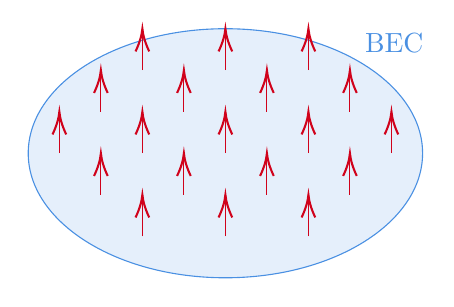
\begin{tikzpicture}[x=0.75pt,y=0.75pt,yscale=-1,xscale=1]
					%uncomment if require: \path (0,300); %set diagram left start at 0, and has height of 300
					
					%Shape: Ellipse [id:dp6222762045043397] 
					\draw  [color={rgb, 255:red, 74; green, 144; blue, 226 }  ,draw opacity=1 ][fill={rgb, 255:red, 74; green, 144; blue, 226 }  ,fill opacity=0.14 ] (15,75) .. controls (15,41.86) and (57.53,15) .. (110,15) .. controls (162.47,15) and (205,41.86) .. (205,75) .. controls (205,108.14) and (162.47,135) .. (110,135) .. controls (57.53,135) and (15,108.14) .. (15,75) -- cycle ;
					%Straight Lines [id:da34596730892301675] 
					\draw [color={rgb, 255:red, 208; green, 2; blue, 27 }  ,draw opacity=1 ]   (30,75) -- (30,57) ;
					\draw [shift={(30,55)}, rotate = 90] [color={rgb, 255:red, 208; green, 2; blue, 27 }  ,draw opacity=1 ][line width=0.75]    (10.93,-3.29) .. controls (6.95,-1.4) and (3.31,-0.3) .. (0,0) .. controls (3.31,0.3) and (6.95,1.4) .. (10.93,3.29)   ;
					%Straight Lines [id:da37008921492668345] 
					\draw [color={rgb, 255:red, 208; green, 2; blue, 27 }  ,draw opacity=1 ]   (70,75) -- (70,57) ;
					\draw [shift={(70,55)}, rotate = 90] [color={rgb, 255:red, 208; green, 2; blue, 27 }  ,draw opacity=1 ][line width=0.75]    (10.93,-3.29) .. controls (6.95,-1.4) and (3.31,-0.3) .. (0,0) .. controls (3.31,0.3) and (6.95,1.4) .. (10.93,3.29)   ;
					%Straight Lines [id:da4058336665062455] 
					\draw [color={rgb, 255:red, 208; green, 2; blue, 27 }  ,draw opacity=1 ]   (110,75) -- (110,57) ;
					\draw [shift={(110,55)}, rotate = 90] [color={rgb, 255:red, 208; green, 2; blue, 27 }  ,draw opacity=1 ][line width=0.75]    (10.93,-3.29) .. controls (6.95,-1.4) and (3.31,-0.3) .. (0,0) .. controls (3.31,0.3) and (6.95,1.4) .. (10.93,3.29)   ;
					%Straight Lines [id:da7816720075968264] 
					\draw [color={rgb, 255:red, 208; green, 2; blue, 27 }  ,draw opacity=1 ]   (150,75) -- (150,57) ;
					\draw [shift={(150,55)}, rotate = 90] [color={rgb, 255:red, 208; green, 2; blue, 27 }  ,draw opacity=1 ][line width=0.75]    (10.93,-3.29) .. controls (6.95,-1.4) and (3.31,-0.3) .. (0,0) .. controls (3.31,0.3) and (6.95,1.4) .. (10.93,3.29)   ;
					%Straight Lines [id:da23143139323089446] 
					\draw [color={rgb, 255:red, 208; green, 2; blue, 27 }  ,draw opacity=1 ]   (190,75) -- (190,57) ;
					\draw [shift={(190,55)}, rotate = 90] [color={rgb, 255:red, 208; green, 2; blue, 27 }  ,draw opacity=1 ][line width=0.75]    (10.93,-3.29) .. controls (6.95,-1.4) and (3.31,-0.3) .. (0,0) .. controls (3.31,0.3) and (6.95,1.4) .. (10.93,3.29)   ;
					%Straight Lines [id:da783377101076965] 
					\draw [color={rgb, 255:red, 208; green, 2; blue, 27 }  ,draw opacity=1 ]   (50,55) -- (50,37) ;
					\draw [shift={(50,35)}, rotate = 90] [color={rgb, 255:red, 208; green, 2; blue, 27 }  ,draw opacity=1 ][line width=0.75]    (10.93,-3.29) .. controls (6.95,-1.4) and (3.31,-0.3) .. (0,0) .. controls (3.31,0.3) and (6.95,1.4) .. (10.93,3.29)   ;
					%Straight Lines [id:da8005324050065074] 
					\draw [color={rgb, 255:red, 208; green, 2; blue, 27 }  ,draw opacity=1 ]   (90,55) -- (90,37) ;
					\draw [shift={(90,35)}, rotate = 90] [color={rgb, 255:red, 208; green, 2; blue, 27 }  ,draw opacity=1 ][line width=0.75]    (10.93,-3.29) .. controls (6.95,-1.4) and (3.31,-0.3) .. (0,0) .. controls (3.31,0.3) and (6.95,1.4) .. (10.93,3.29)   ;
					%Straight Lines [id:da3499214572824182] 
					\draw [color={rgb, 255:red, 208; green, 2; blue, 27 }  ,draw opacity=1 ]   (130,55) -- (130,37) ;
					\draw [shift={(130,35)}, rotate = 90] [color={rgb, 255:red, 208; green, 2; blue, 27 }  ,draw opacity=1 ][line width=0.75]    (10.93,-3.29) .. controls (6.95,-1.4) and (3.31,-0.3) .. (0,0) .. controls (3.31,0.3) and (6.95,1.4) .. (10.93,3.29)   ;
					%Straight Lines [id:da9752930602392493] 
					\draw [color={rgb, 255:red, 208; green, 2; blue, 27 }  ,draw opacity=1 ]   (170,55) -- (170,37) ;
					\draw [shift={(170,35)}, rotate = 90] [color={rgb, 255:red, 208; green, 2; blue, 27 }  ,draw opacity=1 ][line width=0.75]    (10.93,-3.29) .. controls (6.95,-1.4) and (3.31,-0.3) .. (0,0) .. controls (3.31,0.3) and (6.95,1.4) .. (10.93,3.29)   ;
					%Straight Lines [id:da8433456625961715] 
					\draw [color={rgb, 255:red, 208; green, 2; blue, 27 }  ,draw opacity=1 ]   (150,35) -- (150,17) ;
					\draw [shift={(150,15)}, rotate = 90] [color={rgb, 255:red, 208; green, 2; blue, 27 }  ,draw opacity=1 ][line width=0.75]    (10.93,-3.29) .. controls (6.95,-1.4) and (3.31,-0.3) .. (0,0) .. controls (3.31,0.3) and (6.95,1.4) .. (10.93,3.29)   ;
					%Straight Lines [id:da052982943814171235] 
					\draw [color={rgb, 255:red, 208; green, 2; blue, 27 }  ,draw opacity=1 ]   (110,35) -- (110,17) ;
					\draw [shift={(110,15)}, rotate = 90] [color={rgb, 255:red, 208; green, 2; blue, 27 }  ,draw opacity=1 ][line width=0.75]    (10.93,-3.29) .. controls (6.95,-1.4) and (3.31,-0.3) .. (0,0) .. controls (3.31,0.3) and (6.95,1.4) .. (10.93,3.29)   ;
					%Straight Lines [id:da03833569921972457] 
					\draw [color={rgb, 255:red, 208; green, 2; blue, 27 }  ,draw opacity=1 ]   (70,35) -- (70,17) ;
					\draw [shift={(70,15)}, rotate = 90] [color={rgb, 255:red, 208; green, 2; blue, 27 }  ,draw opacity=1 ][line width=0.75]    (10.93,-3.29) .. controls (6.95,-1.4) and (3.31,-0.3) .. (0,0) .. controls (3.31,0.3) and (6.95,1.4) .. (10.93,3.29)   ;
					%Straight Lines [id:da1357054689112429] 
					\draw [color={rgb, 255:red, 208; green, 2; blue, 27 }  ,draw opacity=1 ]   (50,95) -- (50,77) ;
					\draw [shift={(50,75)}, rotate = 90] [color={rgb, 255:red, 208; green, 2; blue, 27 }  ,draw opacity=1 ][line width=0.75]    (10.93,-3.29) .. controls (6.95,-1.4) and (3.31,-0.3) .. (0,0) .. controls (3.31,0.3) and (6.95,1.4) .. (10.93,3.29)   ;
					%Straight Lines [id:da15858972665660132] 
					\draw [color={rgb, 255:red, 208; green, 2; blue, 27 }  ,draw opacity=1 ]   (90,95) -- (90,77) ;
					\draw [shift={(90,75)}, rotate = 90] [color={rgb, 255:red, 208; green, 2; blue, 27 }  ,draw opacity=1 ][line width=0.75]    (10.93,-3.29) .. controls (6.95,-1.4) and (3.31,-0.3) .. (0,0) .. controls (3.31,0.3) and (6.95,1.4) .. (10.93,3.29)   ;
					%Straight Lines [id:da04221706619273946] 
					\draw [color={rgb, 255:red, 208; green, 2; blue, 27 }  ,draw opacity=1 ]   (130,95) -- (130,77) ;
					\draw [shift={(130,75)}, rotate = 90] [color={rgb, 255:red, 208; green, 2; blue, 27 }  ,draw opacity=1 ][line width=0.75]    (10.93,-3.29) .. controls (6.95,-1.4) and (3.31,-0.3) .. (0,0) .. controls (3.31,0.3) and (6.95,1.4) .. (10.93,3.29)   ;
					%Straight Lines [id:da95599164501034] 
					\draw [color={rgb, 255:red, 208; green, 2; blue, 27 }  ,draw opacity=1 ]   (170,95) -- (170,82.75) -- (170,77) ;
					\draw [shift={(170,75)}, rotate = 90] [color={rgb, 255:red, 208; green, 2; blue, 27 }  ,draw opacity=1 ][line width=0.75]    (10.93,-3.29) .. controls (6.95,-1.4) and (3.31,-0.3) .. (0,0) .. controls (3.31,0.3) and (6.95,1.4) .. (10.93,3.29)   ;
					%Straight Lines [id:da2542202779018402] 
					\draw [color={rgb, 255:red, 208; green, 2; blue, 27 }  ,draw opacity=1 ]   (150,115) -- (150,97) ;
					\draw [shift={(150,95)}, rotate = 90] [color={rgb, 255:red, 208; green, 2; blue, 27 }  ,draw opacity=1 ][line width=0.75]    (10.93,-3.29) .. controls (6.95,-1.4) and (3.31,-0.3) .. (0,0) .. controls (3.31,0.3) and (6.95,1.4) .. (10.93,3.29)   ;
					%Straight Lines [id:da9669444297206891] 
					\draw [color={rgb, 255:red, 208; green, 2; blue, 27 }  ,draw opacity=1 ]   (110,115) -- (110,97) ;
					\draw [shift={(110,95)}, rotate = 90] [color={rgb, 255:red, 208; green, 2; blue, 27 }  ,draw opacity=1 ][line width=0.75]    (10.93,-3.29) .. controls (6.95,-1.4) and (3.31,-0.3) .. (0,0) .. controls (3.31,0.3) and (6.95,1.4) .. (10.93,3.29)   ;
					%Straight Lines [id:da021875867656255044] 
					\draw [color={rgb, 255:red, 208; green, 2; blue, 27 }  ,draw opacity=1 ]   (70,115) -- (70,97) ;
					\draw [shift={(70,95)}, rotate = 90] [color={rgb, 255:red, 208; green, 2; blue, 27 }  ,draw opacity=1 ][line width=0.75]    (10.93,-3.29) .. controls (6.95,-1.4) and (3.31,-0.3) .. (0,0) .. controls (3.31,0.3) and (6.95,1.4) .. (10.93,3.29)   ;
					
					% Text Node
					\draw (176,16) node [anchor=north west][inner sep=0.75pt]  [color={rgb, 255:red, 74; green, 144; blue, 226 }  ,opacity=1 ] [align=left] {BEC};
					
					
				\end{tikzpicture}
				
			\end{column}
		\end{columns}
		
	\end{frame}
	\note{
		El sistema experimental es un gas de átomos de Rubidio-87 enfriado hasta cerca del cero absoluto.
		A esa temperatura, todos los átomos caen en el mismo estado cuántico: el BEC está descrito por una sola función de onda macroscópica Ψ.
		Como los átomos tienen espín 1, el parámetro de orden es un espinor con tres componentes: m = +1, 0, -1.
		Al inicio, todos los átomos están en el estado m = +1 (el de menor energía en presencia de un campo magnético, el estado strong-field seeking).
		La fase de espín ζ es lo que va a variar espacialmente para crear el monopolo.
	}
	
	% ==============================================================
	% 8. CREACIÓN DE LA TEXTURA
	% ==============================================================
	\begin{frame}{Textura espinorial}
		
		\begin{columns}[c]
			\begin{column}{0.52\textwidth}
				Campo magnético aplicado:
				\[
				\vb{B} = b_q(x\hat{x}+y\hat{y}-2z\hat{z}) + B_z(t)\hat{z}
				\]
				\vspace{4pt}
				Cero del campo en $\;z = \dfrac{B_z(t)}{2b_q}$
				
				\vspace{10pt}
				\begin{itemize}
					\item Al reducir $B_z(t)$, el cero \textbf{desciende} al BEC
					\item Los espines siguen el campo \textbf{adiabáticamente}
					\item Cada espín rota $\pi - \theta'$ alrededor de $\hat{\varphi}'$
				\end{itemize}
			\end{column}
			\begin{column}{0.45\textwidth}
				\centering
				
				
				\tikzset{every picture/.style={line width=0.75pt}} %set default line width to 0.75pt        
				
				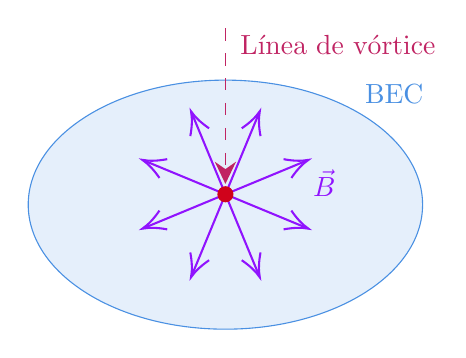
\begin{tikzpicture}[x=0.75pt,y=0.75pt,yscale=-1,xscale=1]
					%uncomment if require: \path (0,180); %set diagram left start at 0, and has height of 180
					
					%Shape: Ellipse [id:dp9751541571698362] 
					\draw  [color={rgb, 255:red, 74; green, 144; blue, 226 }  ,draw opacity=1 ][fill={rgb, 255:red, 74; green, 144; blue, 226 }  ,fill opacity=0.14 ] (15,95) .. controls (15,61.86) and (57.53,35) .. (110,35) .. controls (162.47,35) and (205,61.86) .. (205,95) .. controls (205,128.14) and (162.47,155) .. (110,155) .. controls (57.53,155) and (15,128.14) .. (15,95) -- cycle ;
					%Straight Lines [id:da3701620961778451] 
					\draw [color={rgb, 255:red, 144; green, 19; blue, 254 }  ,draw opacity=1 ][line width=0.75]    (125.8,51.85) -- (94.2,128.15) ;
					\draw [shift={(93.43,130)}, rotate = 292.5] [color={rgb, 255:red, 144; green, 19; blue, 254 }  ,draw opacity=1 ][line width=0.75]    (10.93,-4.9) .. controls (6.95,-2.3) and (3.31,-0.67) .. (0,0) .. controls (3.31,0.67) and (6.95,2.3) .. (10.93,4.9)   ;
					\draw [shift={(126.57,50)}, rotate = 112.5] [color={rgb, 255:red, 144; green, 19; blue, 254 }  ,draw opacity=1 ][line width=0.75]    (10.93,-4.9) .. controls (6.95,-2.3) and (3.31,-0.67) .. (0,0) .. controls (3.31,0.67) and (6.95,2.3) .. (10.93,4.9)   ;
					%Straight Lines [id:da2741119987481083] 
					\draw [color={rgb, 255:red, 144; green, 19; blue, 254 }  ,draw opacity=1 ][line width=0.75]    (125.8,128.15) -- (94.2,51.85) ;
					\draw [shift={(93.43,50)}, rotate = 67.5] [color={rgb, 255:red, 144; green, 19; blue, 254 }  ,draw opacity=1 ][line width=0.75]    (10.93,-4.9) .. controls (6.95,-2.3) and (3.31,-0.67) .. (0,0) .. controls (3.31,0.67) and (6.95,2.3) .. (10.93,4.9)   ;
					\draw [shift={(126.57,130)}, rotate = 247.5] [color={rgb, 255:red, 144; green, 19; blue, 254 }  ,draw opacity=1 ][line width=0.75]    (10.93,-4.9) .. controls (6.95,-2.3) and (3.31,-0.67) .. (0,0) .. controls (3.31,0.67) and (6.95,2.3) .. (10.93,4.9)   ;
					%Straight Lines [id:da637181877963864] 
					\draw [color={rgb, 255:red, 144; green, 19; blue, 254 }  ,draw opacity=1 ][line width=0.75]    (148.15,105.8) -- (71.85,74.2) ;
					\draw [shift={(70,73.43)}, rotate = 22.5] [color={rgb, 255:red, 144; green, 19; blue, 254 }  ,draw opacity=1 ][line width=0.75]    (10.93,-4.9) .. controls (6.95,-2.3) and (3.31,-0.67) .. (0,0) .. controls (3.31,0.67) and (6.95,2.3) .. (10.93,4.9)   ;
					\draw [shift={(150,106.57)}, rotate = 202.5] [color={rgb, 255:red, 144; green, 19; blue, 254 }  ,draw opacity=1 ][line width=0.75]    (10.93,-4.9) .. controls (6.95,-2.3) and (3.31,-0.67) .. (0,0) .. controls (3.31,0.67) and (6.95,2.3) .. (10.93,4.9)   ;
					%Straight Lines [id:da008637001499207875] 
					\draw [color={rgb, 255:red, 144; green, 19; blue, 254 }  ,draw opacity=1 ][line width=0.75]    (71.85,105.8) -- (148.15,74.2) ;
					\draw [shift={(150,73.43)}, rotate = 157.5] [color={rgb, 255:red, 144; green, 19; blue, 254 }  ,draw opacity=1 ][line width=0.75]    (10.93,-4.9) .. controls (6.95,-2.3) and (3.31,-0.67) .. (0,0) .. controls (3.31,0.67) and (6.95,2.3) .. (10.93,4.9)   ;
					\draw [shift={(70,106.57)}, rotate = 337.5] [color={rgb, 255:red, 144; green, 19; blue, 254 }  ,draw opacity=1 ][line width=0.75]    (10.93,-4.9) .. controls (6.95,-2.3) and (3.31,-0.67) .. (0,0) .. controls (3.31,0.67) and (6.95,2.3) .. (10.93,4.9)   ;
					
					%Shape: Ellipse [id:dp6668158525443336] 
					\draw  [color={rgb, 255:red, 208; green, 2; blue, 27 }  ,draw opacity=1 ][fill={rgb, 255:red, 208; green, 2; blue, 27 }  ,fill opacity=1 ] (106.39,90) .. controls (106.39,88.01) and (108.01,86.39) .. (110,86.39) .. controls (111.99,86.39) and (113.61,88.01) .. (113.61,90) .. controls (113.61,91.99) and (111.99,93.61) .. (110,93.61) .. controls (108.01,93.61) and (106.39,91.99) .. (106.39,90) -- cycle ;
					%Straight Lines [id:da6358756922105985] 
					\draw [color={rgb, 255:red, 192; green, 36; blue, 99 }  ,draw opacity=1 ] [dash pattern={on 4.5pt off 4.5pt}]  (110,10) -- (110,82) ;
					\draw [shift={(110,85)}, rotate = 270] [fill={rgb, 255:red, 192; green, 36; blue, 99 }  ,fill opacity=1 ][line width=0.08]  [draw opacity=0] (10.72,-5.15) -- (0,0) -- (10.72,5.15) -- (7.12,0) -- cycle    ;
					
					% Text Node
					\draw (176,36) node [anchor=north west][inner sep=0.75pt]  [color={rgb, 255:red, 74; green, 144; blue, 226 }  ,opacity=1 ] [align=left] {BEC};
					% Text Node
					\draw (116,12) node [anchor=north west][inner sep=0.75pt]  [color={rgb, 255:red, 192; green, 36; blue, 99 }  ,opacity=1 ] [align=left] {Línea de vórtice};
					% Text Node
					\draw (151,77) node [anchor=north west][inner sep=0.75pt]  [color={rgb, 255:red, 144; green, 19; blue, 254 }  ,opacity=1 ] [align=left] {$\displaystyle \vec{B}$};
					
					
				\end{tikzpicture}
				
			\end{column}
		\end{columns}
		
	\end{frame}
	\note{
		El campo cuadrupolar tiene un punto cero: el punto donde B = 0 exactamente.
		Inicialmente ese cero está por encima del condensado (lejos de él).
		Al reducir B_z lentamente, el cero desciende y entra al condensado.
		Los átomos siguen el campo adiabáticamente: cada espín rota para apuntar en la dirección del campo local en cada instante.
		El resultado es una textura tipo «erizo» (hedgehog): los espines apuntan en todas direcciones desde el cero del campo.
		Junto con esto, aparece automáticamente una línea de vórtice (densidad nula) desde el cero hacia la superficie del condensado.
	}
	
	% ==============================================================
	% 9. EL ESPINOR RESULTADO
	% ==============================================================
	\begin{frame}{Textura espinorial 2}
		
		\[
		\zeta(\theta',\phi') =
		\begin{pmatrix}
			\dfrac{1-\cos\theta'}{2}\\[10pt]
			-\dfrac{e^{i\phi'}\sin\theta'}{\sqrt{2}}\\[10pt]
			\dfrac{e^{2i\phi'}(1+\cos\theta')}{2}
		\end{pmatrix}
		\]
		
		\vspace{10pt}
		\centering
		\small
		\begin{tabular}{ccc}
			$\theta' \to 0$ (arriba del cero) &
			$\theta' = \pi/2$ (ecuador) &
			$\theta' \to \pi$ (abajo del cero) \\[4pt]
			$\zeta \to (0,\,0,\,1)^T$ &
			$\zeta \to (0,\,-e^{i\phi'}/\sqrt{2},\,0)^T$ &
			$\zeta \to (1,\,0,\,0)^T$ \\
			espín $m=-1$ & espín $m=0$ & espín $m=+1$
		\end{tabular}
		
	\end{frame}
	\note{
		Este es el espinor que se obtiene al rotar el estado inicial (1,0,0) por un ángulo π-θ' alrededor del eje azimuthal.
		Se puede verificar que está normalizado: la suma de los cuadrados de los módulos es 1.
		El punto clave: la componente m=-1 lleva la fase e^{2iφ'}, que da un enrolamiento doble al dar una vuelta completa alrededor del eje z'.
		Abajo del monopolo (θ' → π), el espinor es (1,0,0) — exactamente igual al estado inicial, sin haber cambiado: esos átomos nunca sintieron pasar el cero.
		Esta estructura del espinor es lo que va a generar la velocidad superfluida y el campo sintético.
	}
	\begin{frame}
		
	\begin{figure}
			\centering
			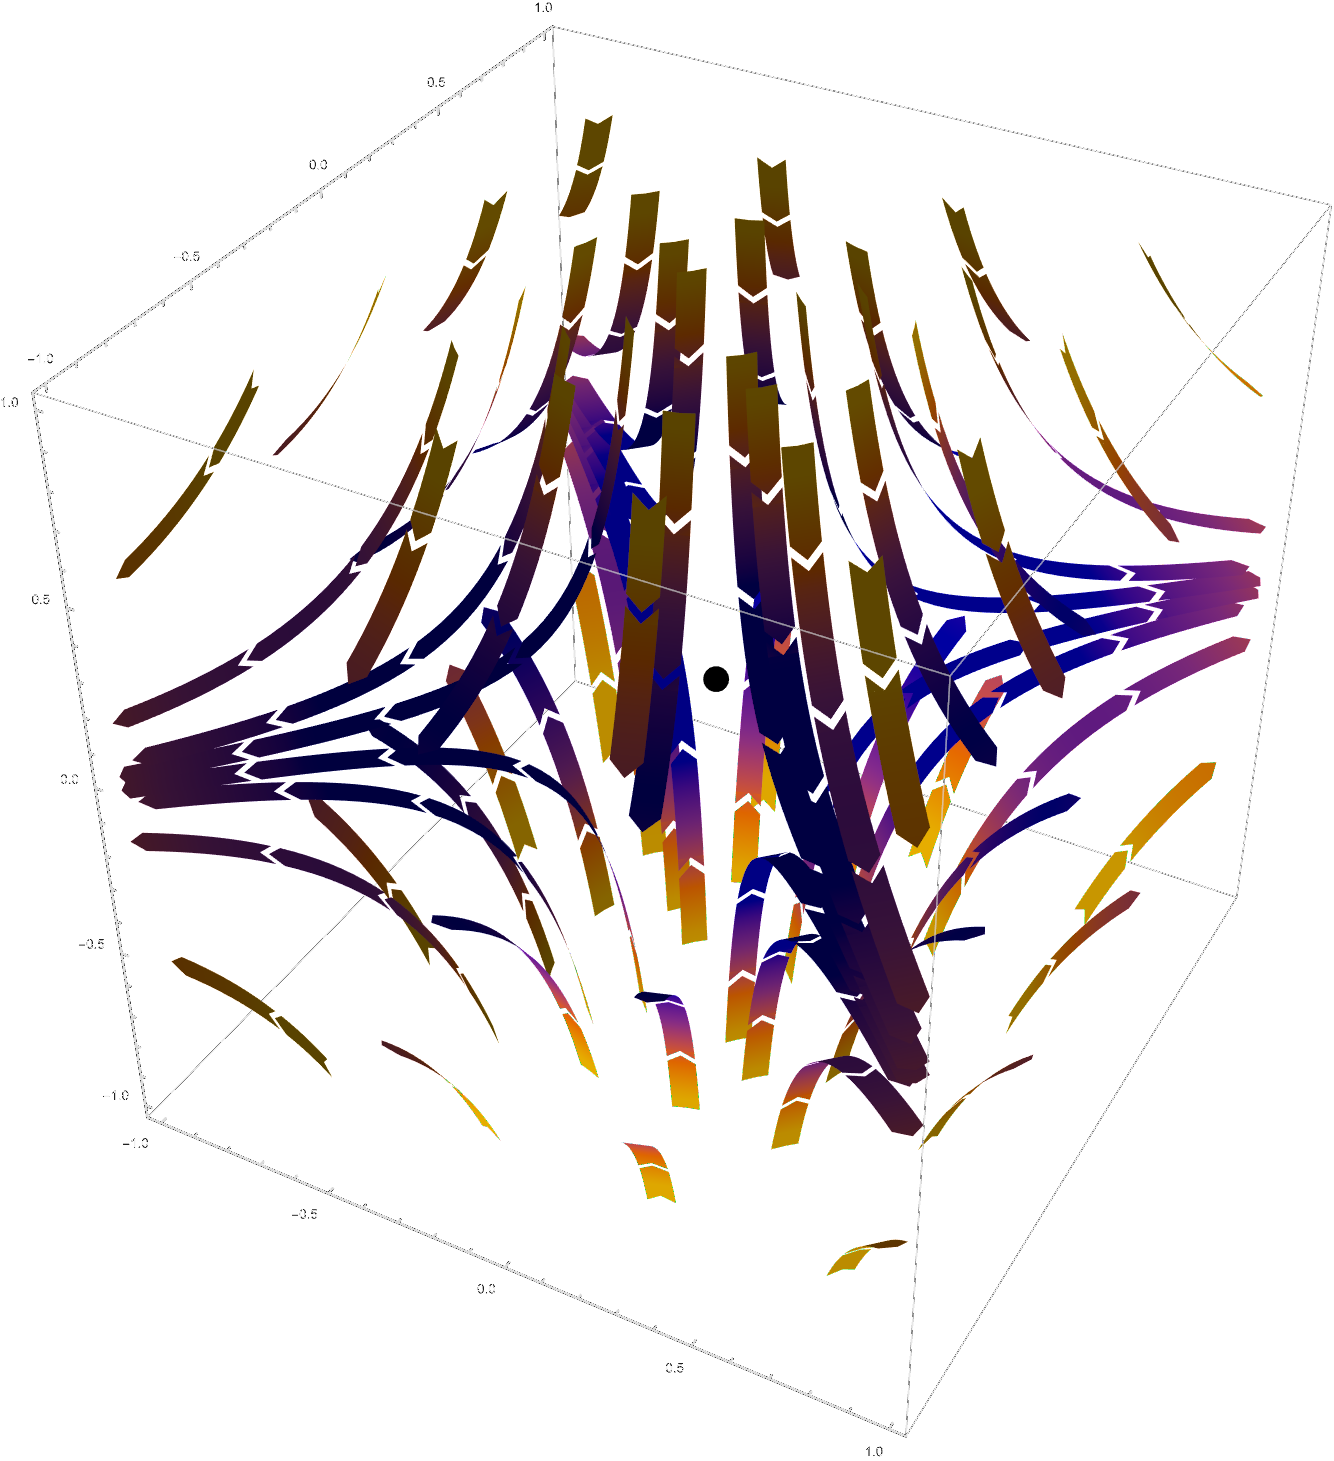
\includegraphics[width=0.47\linewidth]{campoVec1} ~~~
			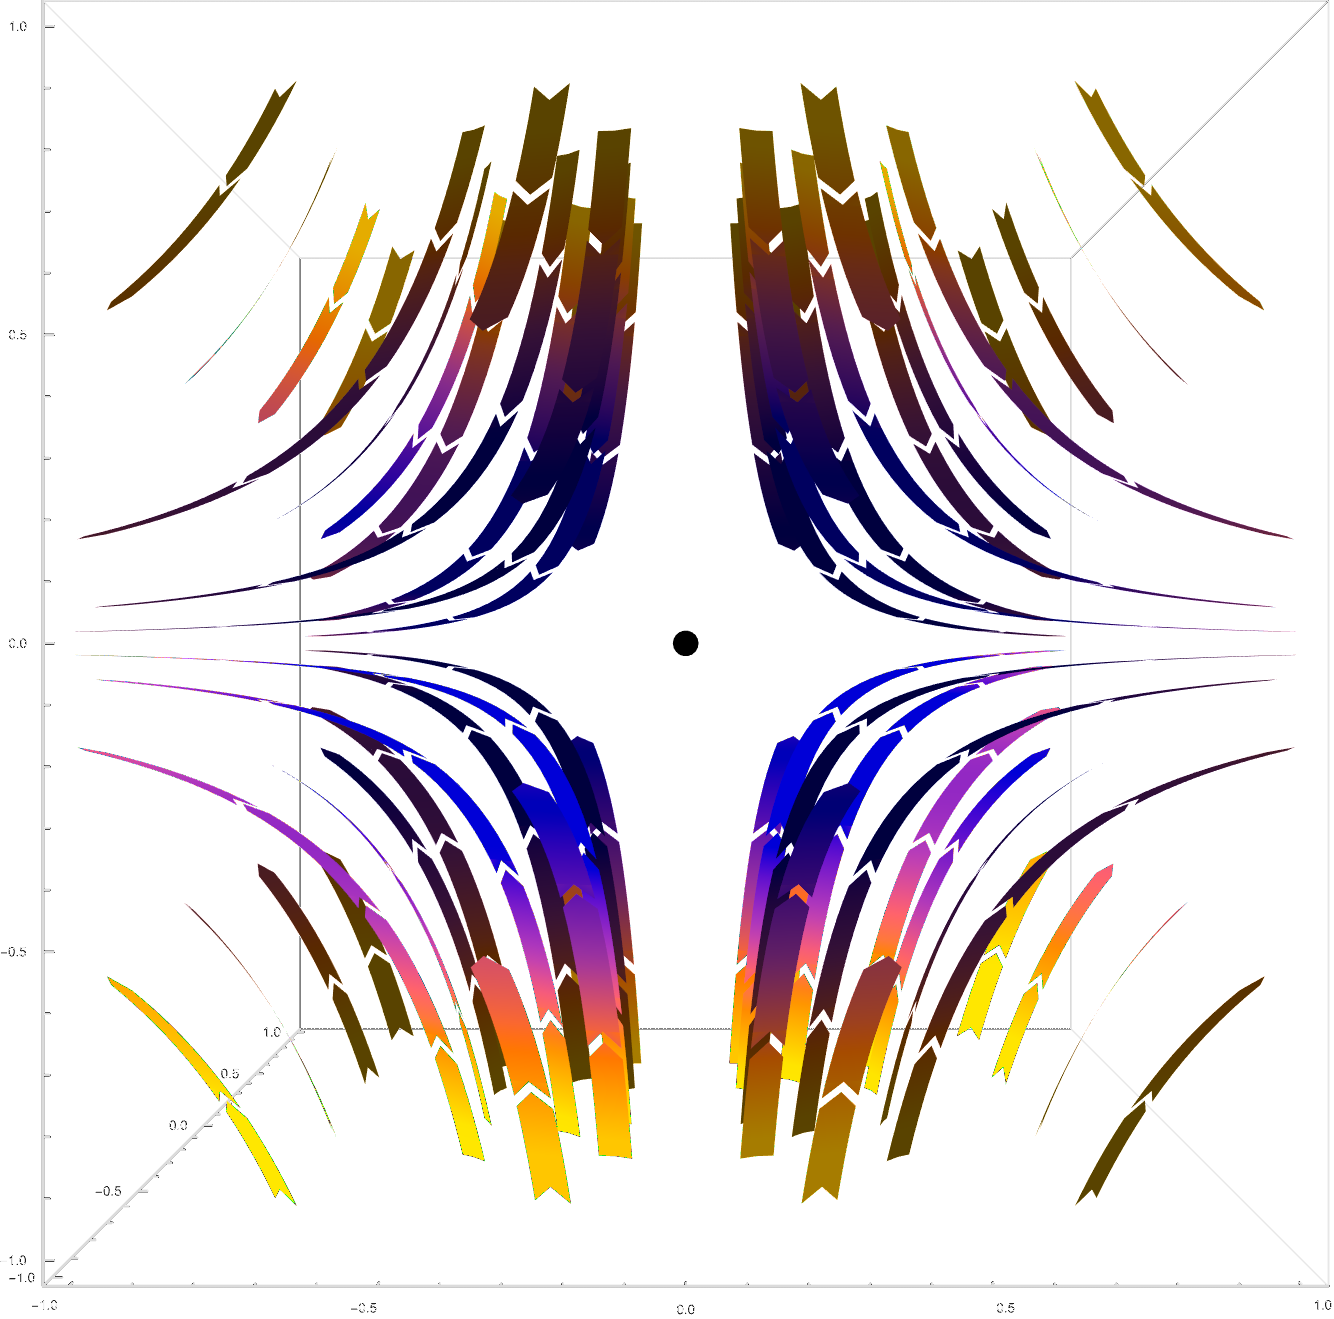
\includegraphics[width=0.47\linewidth]{campoVec2}
			\label{fig:campovec1}
		\end{figure}
	\end{frame}
	
	% ==============================================================
	% 10. LA VELOCIDAD SUPERFLUIDA
	% ==============================================================
	\begin{frame}{Velocidad superfluida}
		
		\begin{columns}[c]
			\begin{column}{0.5\textwidth}
				La variación espacial del espinor genera una fase geométrica.
				La velocidad superfluida es el gradiente de esa fase:
				\[
				v_s^{\varphi'} = \frac{\hbar}{M}\,
				\mathrm{Im}\!\left(\zeta^\dagger\frac{\partial\zeta}{\partial\phi'}\right)
				\frac{1}{r'\sin\theta'}
				\]
				\[
				\boxed{v_s^{\varphi'} = \frac{\hbar}{M}\,\frac{1+\cos\theta'}{r'\sin\theta'}}
				\]
			\end{column}
			\begin{column}{0.5\textwidth}
				\begin{figure}
					\centering
					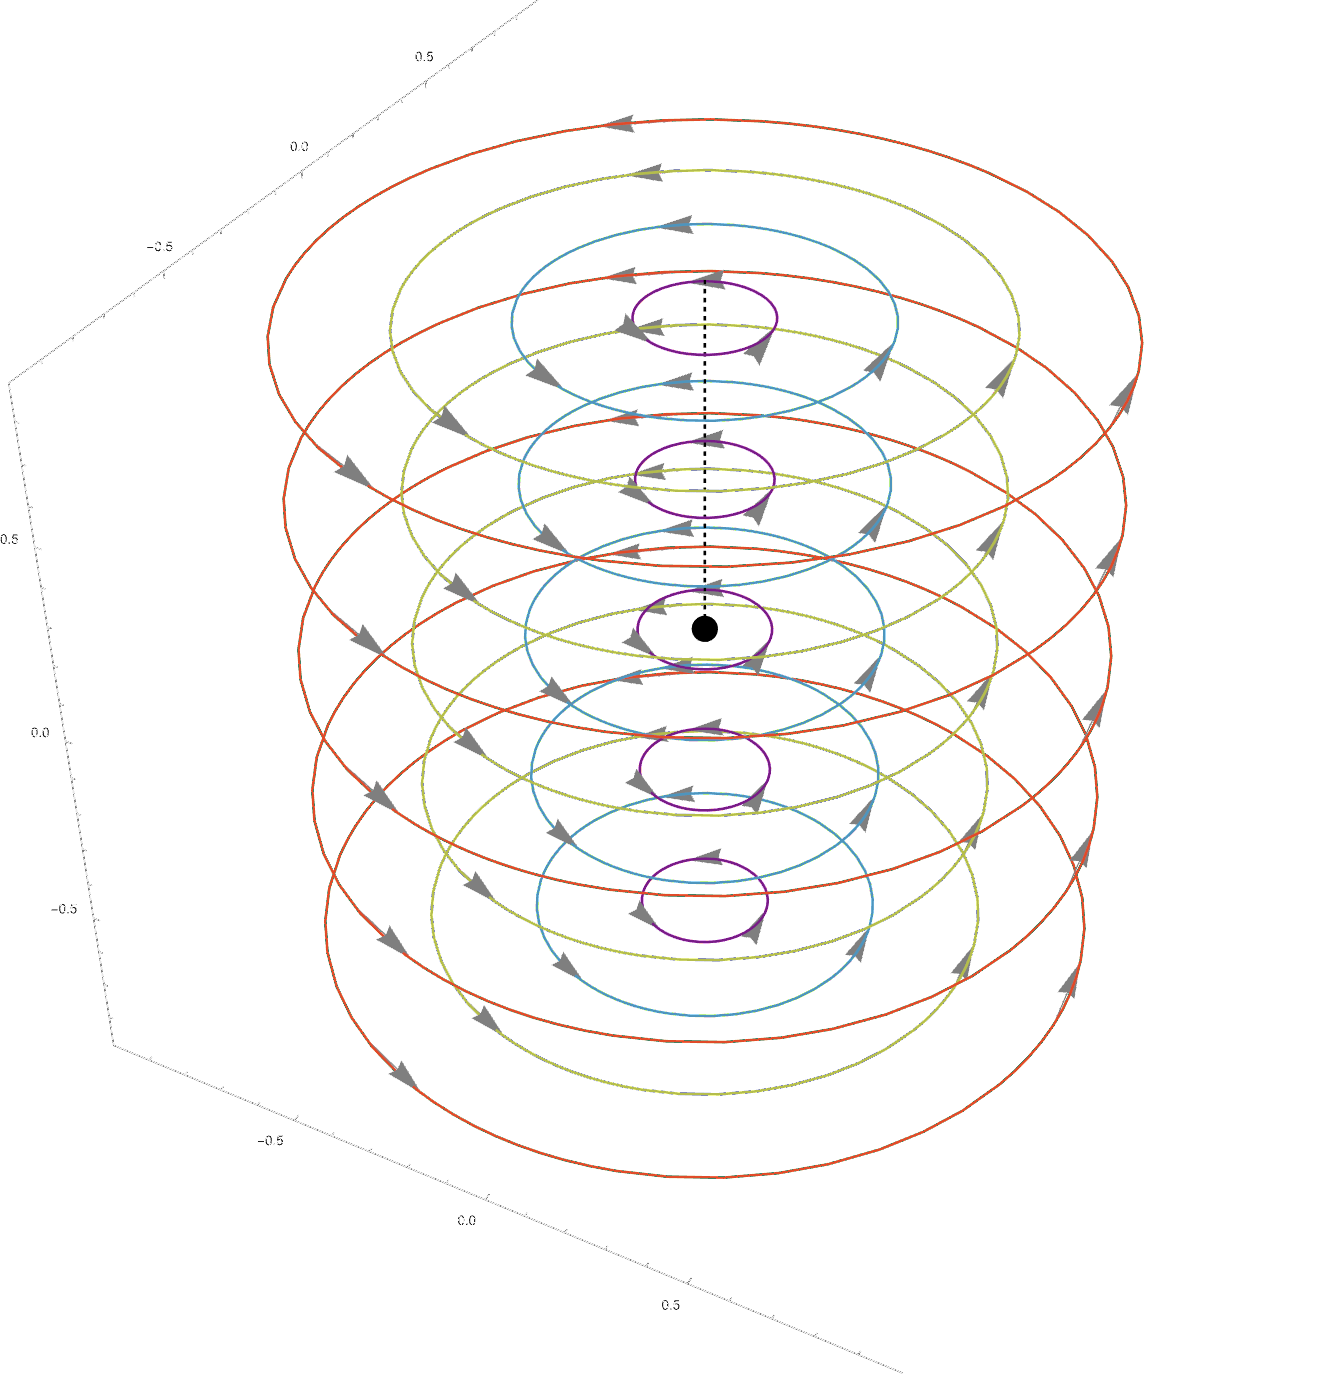
\includegraphics[width=\linewidth]{velocidades}
					\label{fig:velocidades}
				\end{figure}
			\end{column}
		\end{columns}
		
	\end{frame}
	\note{
		En un BEC espinorial, la velocidad superfluida tiene una contribución de la variación espacial del espinor: la fase de Berry.
		Concretamente, como el espinor cambia de un punto a otro (la textura), al moverse por el condensado se acumula una fase geométrica.
		La fórmula muestra que vs es puramente azimutal: los átomos circulan alrededor del eje z'.
		La velocidad diverge como 1/sin(θ') al acercarse al eje z' (θ'→0): esto es el vórtice.
		En el eje -z' (θ'→π), la velocidad va a cero suavemente: no hay vórtice allí.
	}
	
	% ==============================================================
	% 11. LA VORTICIDAD
	% ==============================================================
	\begin{frame}{Vorticidad}
		
		\[
		\Omega = \ro\vb{v}_s =
		\underbrace{-\frac{\hbar}{Mr'^2}\,\rph}_{\displaystyle\text{término monopolar}}
		\;+\;
		\underbrace{\frac{4\pi\hbar}{M}\,\delta(x')\delta(y')\,\Theta(z')\,\rph}_{\displaystyle\text{línea de vórtice (\textit{Dirac string})}}
		\]
		
		\vspace{14pt}
		\begin{columns}[c]
			\begin{column}{0.48\textwidth}
				\begin{block}{\centering Primer término}
					\centering Campo radial $\propto 1/r'^2$\\
					irradia desde el origen
				\end{block}
			\end{column}
			\begin{column}{0.48\textwidth}
				\begin{block}{\centering Segundo término}
					\centering $\delta(x')\delta(y')$: concentrado en el eje $z'$\\
					$\Theta(z')$: solo para $z'>0$
				\end{block}
			\end{column}
		\end{columns}
		
	\end{frame}
	\note{
		Tomamos el curl de vs para obtener la vorticidad.
		El primer término aparece del cálculo directo: es un campo radial tipo 1/r², que irradia desde el origen (el monopolo).
		El segundo término aparece por la singularidad del campo de velocidades en el eje z' para z' > 0. Es una función delta que concentra toda la vorticidad en esa línea — la línea de vórtice.
		El factor Θ(z') (función escalón de Heaviside) indica que la línea de vórtice solo existe para z' > 0: desde el monopolo hacia arriba, hasta la superficie del condensado.
		Esta es exactamente la estructura matemática que Dirac describió: monopolo + Dirac string semisinfina adjunta.
	}
	
	% ==============================================================
	% 12. EL RESULTADO PRINCIPAL — CAMPO SINTÉTICO
	% ==============================================================
	\begin{frame}{Campo magnético sintético}
		
		\[
		\vb{B}^* = \ro\vb{A}^* = -M\Omega
		\]
		
		\vspace{6pt}
		El término de la \textit{Dirac string} es dependiente de \textit{gauge}: se anula.
		
		\vspace{14pt}
		\centering
		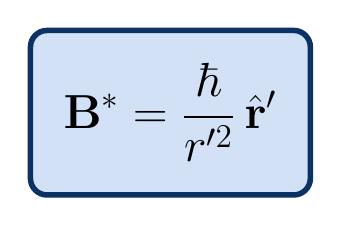
\begin{tikzpicture}
			\node[draw=azul,line width=2pt,rounded corners=6pt,
			fill=azulclaro,inner sep=12pt,font=\LARGE\bfseries] {
				$\displaystyle\vb{B}^* = \frac{\hbar}{r'^2}\,\rph$
			};
		\end{tikzpicture}
		
		\vspace{12pt}
		\normalsize
		\[
		\textbf{Idéntico a }\;\vb{B} = \frac{g}{r^2}\rh\;\textbf{ con }\;g\to\hbar
		\]
		
	\end{frame}
	\note{
		Este es el resultado central del paper.
		Definimos el potencial vectorial sintético como A* = -(M/ℏ)vs, y su curl da B*.
		El término de la Dirac string en B* es dependiente de gauge: usando la construcción de Wu-Yang (dos parches de gauge), se puede eliminar.
		Lo que queda es el campo monopolar: B* = ℏ r̂'/r'^2.
		Esto es exactamente la forma del campo de un monopolo magnético real, con g → ℏ.
		Este campo actúa sobre el condensado a través de la fase de Berry, no a través de la fuerza de Lorentz (los átomos son neutros).
	}
	
	% ==============================================================
	% 13. LA CONDICIÓN DE DIRAC VERIFICADA
	% ==============================================================
	\begin{frame}{Condición de Dirac}
		
		\begin{columns}[c]
			\begin{column}{0.5\textwidth}
				Acumulación de fase alrededor del eje $+z'$:
				\[
				\Delta\phi = \frac{M}{\hbar}\oint\vb{v}_s\cdot d\vb{l}
				= 2\pi(1+\cos\theta')
				\]
				En $\theta'\to 0$ (sobre el monopolo):
				\[
				\boxed{\Delta\phi = 4\pi}
				\]
			\end{column}
			\begin{column}{0.47\textwidth}
				\begin{block}{\centering Condición de Dirac}
					\[
					e^{i\,\Delta\phi} = e^{i\cdot 4\pi} = 1
					\]
					La línea de vórtice ($4\pi$ winding)\\
					es la \textbf{Dirac string}: no observable.
				\end{block}
				\vspace{6pt}
				\begin{block}{\centering Confirmación experimental}
					La línea se \textbf{divide en dos} tras ${\sim}10\,\mathrm{ms}$\\
					{\small (vórtice $4\pi$ es inestable)}
				\end{block}
			\end{column}
		\end{columns}
		
	\end{frame}
	\note{
		La condición de Dirac dice que la fase acumulada al rodear la Dirac string debe ser un múltiplo de 2π para que la cuerda sea no observable.
		Aquí Δφ = 4π = 2×2π, así que e^{i·4π} = 1: se cumple exactamente.
		Esto confirma que la línea de vórtice juega el papel de la Dirac string.
		La confirmación experimental del 4π es que un vórtice doblemente cuantizado (4π = 2×2π) es inestable: se divide espontáneamente en dos vórtices simples.
		Esto se observa directamente en la Figura S1 del artículo: después de ~10 ms, una sola línea de densidad nula se convierte en dos.
	}
	
	% ==============================================================
	% 14. EVIDENCIA EXPERIMENTAL — FIGURA
	% ==============================================================
	\begin{frame}{Evidencia experimental}
		
		\begin{columns}[c]
			\begin{column}{0.55\textwidth}
				%% ---------------------------------------------------------
				%% Insertar aquí la Figura 3 del artículo:
				%%   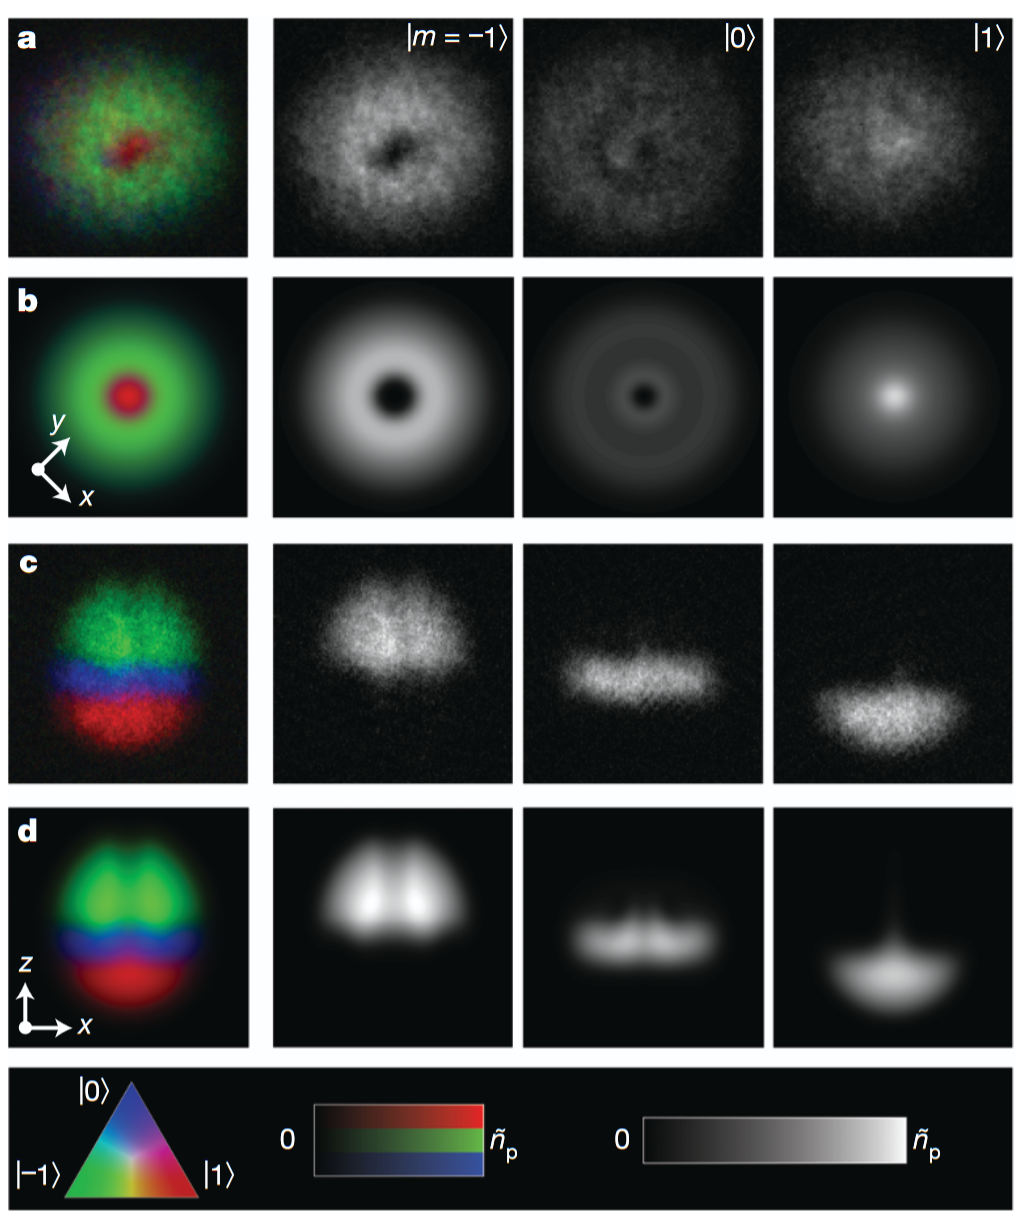
\includegraphics[width=\textwidth]{fig3}
				%% Exportar como fig3.png desde el PDF del artículo
				%% ---------------------------------------------------------
				\centering
				
				\begin{figure}
					\centering
					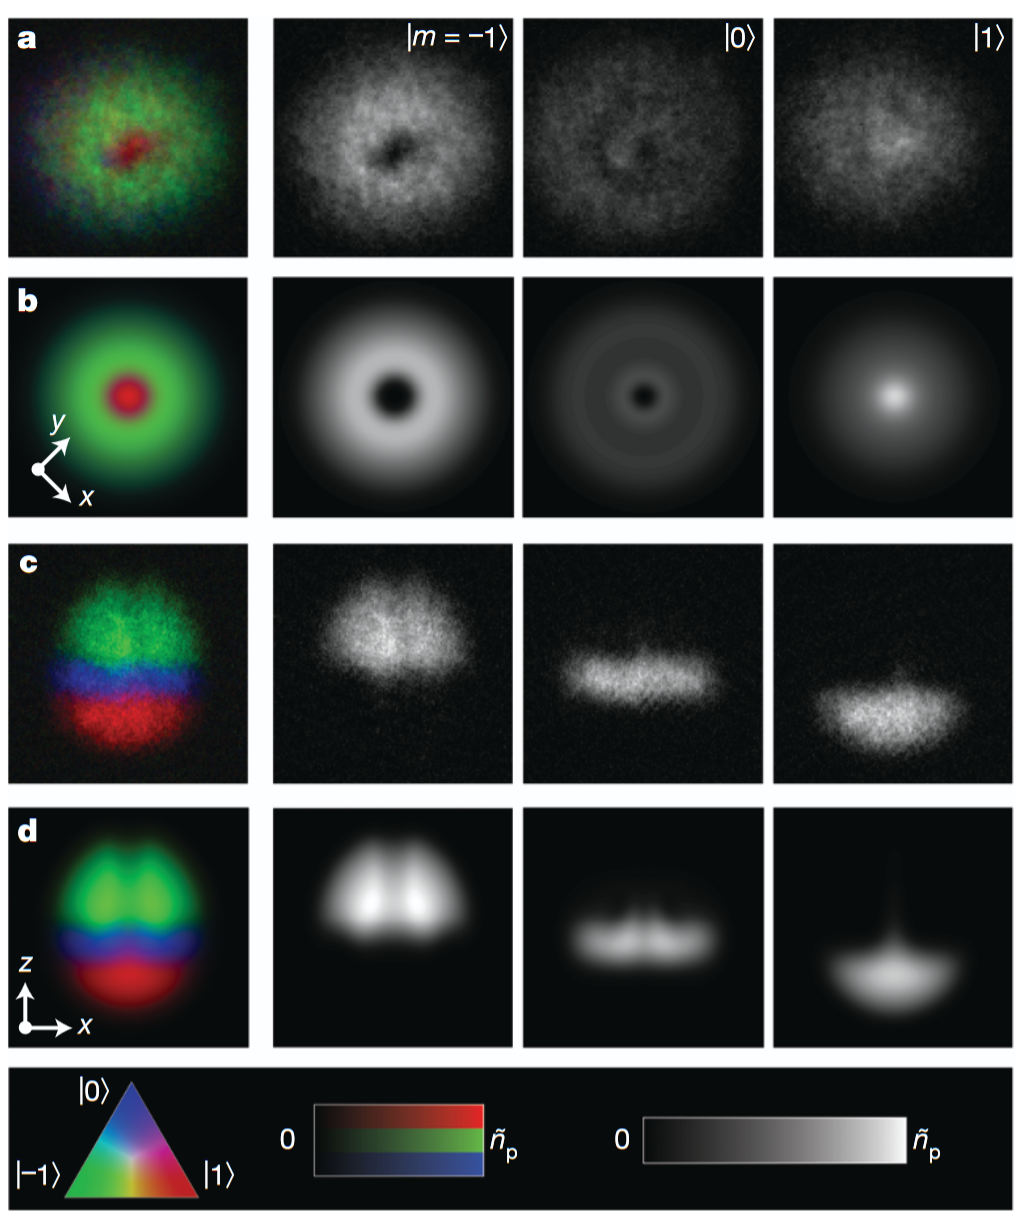
\includegraphics[width=.7\linewidth]{fig3}
					\caption{M. W. Ray, E. Ruokokoski, S. Kandel, M. Möttönen, and D. S. Hall, Nature 505, 657 (2014).}
					\label{fig:fig3}
				\end{figure}
			\end{column}
			\begin{column}{0.45\textwidth}
				Densidades de los tres componentes de espín con el monopolo en el centro. (a,c): Experimento. (b,d): Simulación.
				\begin{itemize}
					\item Línea de densidad nula visible
					\item Termina dentro del condensado
					\item Simulaciones sin parámetros libres
					\item Distribución de espines coincide con la simulación
				\end{itemize}
			\end{column}
		\end{columns}
		
	\end{frame}
	\note{
		Mostrar la Figura 3 del paper.
		Las imágenes muestran las densidades de columna de los tres componentes de espín (m = +1, 0, -1) vistas desde dos ángulos.
		La línea de densidad nula (el vórtice / Dirac string) aparece como un agujero en la densidad de los componentes m = -1 y m = 0.
		Crucialmente, la línea TERMINA DENTRO del condensado: eso es la evidencia del monopolo en su extremo.
		El acuerdo cuantitativo con la simulación numérica (sin parámetros ajustables) valida completamente la interpretación.
	}
	
	% ==============================================================
	% 15. CONEXIÓN CON EL CURSO
	% ==============================================================
	\begin{frame}{Conexión con el curso}
		
		\centering
		\begin{itemize}
			\item $\di\vb{B}=0$ y $\vb{B}=\ro\vb{A}$
			\item Teorema de Stokes
			\item Teorema de Gauss
			\item Ley de Faraday
			\item Invarianza de gauge
			\item Efecto Aharonov-Bohm
		\end{itemize}
		\begin{tabular}{lll}
%			\hrule
%			\textbf{Herramienta} & \textbf{Rol en el artículo} & \\
%			\hrule
%			$\di\vb{B}=0$ y $\vb{B}=\ro\vb{A}$ & Origen del problema & \\[4pt]
%			Invarianza de gauge & La Dirac string es no física & \\[4pt]
%			Teorema de Stokes & $\Delta\phi = \iint\vb{\Omega}\cdot d\vb{A}$ & \\[4pt]
%			Teorema de Gauss & Flujo monopolar $\oint\vb{B}^*\cdot d\vb{A} = 4\pi\hbar$ & \\[4pt]
%			Efecto Aharonov-Bohm & Condición $e^{i\Delta\phi}=1$ & \\[4pt]
%			Ley de Faraday & $\ro\vb{E}^* = -\partial\vb{B}^*/\partial t$ & \\
%			\hrule
		\end{tabular}
		
		\vspace{12pt}
		\small La construcción de Dirac puede desarrollarse casi completamente\\
		con las herramientas del curso.
		
	\end{frame}
	\note{
		Este es el slide más importante para la evaluación: la conexión explícita con el curso.
		Recorrer la tabla brevemente:
		- La identidad vectorial ∇·(∇×A) ≡ 0 es lo que hace imposible el monopolo con A global.
		- La invarianza de gauge explica por qué la dirección de la Dirac string no es observable.
		- El teorema de Stokes es cómo conectamos el enrolamiento de fase con el flujo de vorticidad.
		- El teorema de Gauss cuantifica el flujo del campo monopolar.
		- El efecto Aharonov-Bohm (que vimos en el curso) es lo que hace la cuerda no observable y da la cuantización de Dirac.
		- Faraday aparece en el campo eléctrico sintético que se genera cuando el monopolo se mueve.
		Destacar que Dirac (1931) llegó a todo esto con electrodinámica clásica más un argumento cuántico mínimo.
	}
	
	% ==============================================================
	% 16. DISCUSIÓN CRÍTICA
	% ==============================================================
	\begin{frame}{Discusión}
		
		\begin{columns}[T]
			\begin{column}{0.47\textwidth}
				\begin{alertblock}{Limitaciones}
					\begin{itemize}
						\item Campo \textbf{sintético}, no electromagnético
						\item No afecta a cargas externas
						\item No es el estado base (decae)
						\item Condiciones extremas ($T \approx 0$)
					\end{itemize}
				\end{alertblock}
			\end{column}
			\begin{column}{0.5\textwidth}
				\begin{block}{Se verificó:}
					\begin{itemize}
						\item $\vb{B}^* = \hbar \, \rph/r'^2$
						\item Dirac string con $\Delta\phi = 4\pi$
						\item $e^{i\cdot 4\pi} = 1$
						\item Dirección de la cuerda: de gauge
						\item Extremo de la cuerda: gauge-invariante
						\item Sin parámetros libres
					\end{itemize}
				\end{block}
			\end{column}
		\end{columns}
		
	\end{frame}
	\note{
		Las limitaciones son reales y el propio artículo las reconoce.
		El campo B* no es el campo electromagnético: los átomos son neutros, no hay fuerza de Lorentz.
		El monopolo no es estable: fue creado en un estado excitado y eventualmente decae.
		Sin embargo, lo que se verificó cubre TODOS los elementos de la construcción teórica de Dirac.
		El punto importante para la conclusión: la pregunta de si existen monopolos «reales» en el campo electromagnético sigue abierta.
		Pero la estructura matemática y física de Dirac fue completamente realizada en este sistema.
	}
	
	% ==============================================================
	% 17. CONCLUSIÓN
	% ==============================================================
	\begin{frame}{Conclusión}
		
		\centering
		\vspace{8pt}
		
		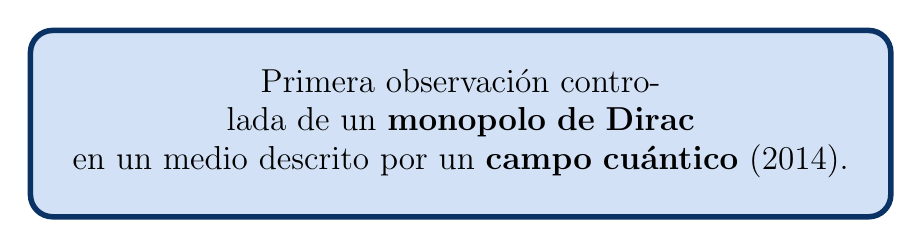
\begin{tikzpicture}
			\node[draw=azul,line width=2pt,rounded corners=8pt,
			fill=azulclaro,inner sep=14pt,text width=0.82\textwidth,
			align=center,font=\large] {
				Primera observación controlada de un \textbf{monopolo de Dirac}\\
				en un medio descrito por un \textbf{campo cuántico} (2014).
			};
		\end{tikzpicture}

		
	\end{frame}
	\note{
		Cerrar con energía.
		Este artículo cierra un ciclo de 83 años entre la teoría de Dirac (1931) y la primera observación en un campo cuántico (2014).
		Lo que hace este resultado importante no es solo el «hemos creado un monopolo» — es que los conceptos del curso (potencial vectorial, gauge, flujo, Aharonov-Bohm) son suficientemente poderosos para guiar el diseño de este experimento y predecir cada detalle de lo que se observa.
		La frase de cierre: mencionar que la ingeniería de campos sintéticos abre puertas a estudiar monopolos no-Abelianos, efecto Hall cuántico, y otros fenómenos topológicos en sistemas cuánticos controlados.
	}
	
	\appendix
	
	\begin{frame}
		\titlepage
	\end{frame}
	
	\begin{frame}
		\centering
		\Huge
		\vspace{10mm}
		Backup slides
	\end{frame}
	
	
	%--- B1 ---
	\begin{frame}{Derivación de $\mathbf{A}$}
		Flujo a través del casquete esférico hasta ángulo $\theta$:
		\[ \Phi(\theta) = \iint_\text{cap} \frac{g}{r^2}\hat{r}\cdot d\mathbf{A}
		= 2\pi g(1-\cos\theta) \]
		Por Stokes: $\oint \mathbf{A}\cdot d\mathbf{l} = \Phi$, con $|\mathbf{l}| = 2\pi r\sin\theta$:
		\[ A_\phi = \frac{g(1-\cos\theta)}{r\sin\theta}
		\;\;\Rightarrow\;\; \nabla\times\mathbf{A} = \frac{g}{r^2}\hat{r} \]
		Singularidad en $\theta=\pi$: la \textit{Dirac string}.
	\end{frame}
	
	%--- B2 ---
	\begin{frame}{Condición de cuantización de Dirac}
		Fase Aharonov-Bohm al rodear la cuerda (flujo $= 4\pi g$):
		\[ \exp\!\left[\frac{iq}{\hbar c}\oint\mathbf{A}\cdot d\mathbf{l}\right]
		= \exp\!\left[\frac{4\pi i qg}{\hbar c}\right] = 1 \]
		La función de onda del electrón debe ser univaluada:
		\[ \frac{4\pi qg}{\hbar c} = 2\pi n
		\;\;\Rightarrow\;\; \boxed{qg = \frac{n\hbar c}{2}} \]
	\end{frame}
	
	%--- B3 ---
	\begin{frame}{$\Delta\phi = 4\pi$}
		Rotación de $(1,0,0)^T$ por $\pi-\theta'$ alrededor de $\hat{\varphi}'$
		(matrices de Wigner $d^{(1)}$):
		\[ \zeta = \begin{pmatrix}(1-\cos\theta')/2 \\
			-e^{i\phi'}\sin\theta'/\sqrt{2} \\
			e^{2i\phi'}(1+\cos\theta')/2 \end{pmatrix} \]
		La componente $\zeta_{-1}$ lleva fase $e^{2i\phi'}$:
		al dar una vuelta completa en $\phi'$, acumula $4\pi$.\\[6pt]
		En $\theta'\to 0$: $\zeta_{-1}\to 1$ (dominante) $\Rightarrow \Delta\phi = 4\pi$.
	\end{frame}
	
	%--- B4 ---
	\begin{frame}{Fase de Berry $\to$ velocidad superfluida}
		Variación del espinor genera una fase geométrica:
		\[ \zeta^\dagger\frac{\partial\zeta}{\partial\phi'}
		= i(1+\cos\theta') \]
		Velocidad superfluida = gradiente de esa fase:
		\[ v_s^{\phi'} = \frac{\hbar}{M}
		\mathrm{Im}\!\left(\zeta^\dagger\frac{\partial\zeta}{\partial\phi'}\right)
		\frac{1}{r'\sin\theta'}
		= \frac{\hbar}{M}\frac{1+\cos\theta'}{r'\sin\theta'} \]
	\end{frame}
	
	%--- B5 ---
	\begin{frame}{Gauge}
		Bajo $\mathbf{A}^* \to \mathbf{A}^* + \nabla\chi$, la singularidad
		se mueve de dirección.\\[8pt]
		\textbf{Wu-Yang (ref. 20):} usar dos parches de gauge superpuestos
		(hemisferio norte y sur), cada uno con $\mathbf{A}^*$ regular.
		En la superposición, se relacionan por una transformación de gauge.\\[8pt]
		Resultado: \textbf{ninguna} singularidad en $\mathbf{A}^*$, pero la
		línea de vórtice física (densidad nula) permanece.\\[8pt]
%		\centering
%		Gauge-dependiente: dirección de la cuerda.\\
%		Gauge-invariante: el extremo (el monopolo).
	\end{frame}
\end{document}